\chapter{Spatial econometrics to estimate the traffic reduction by transforming office space into housing: the case for Barcelona\textsuperscript{*}}
\chaptermark{Estimating traffic reduction by transforming offices into housing}
\label{ch:ETRCO2H}
\graphicspath{{chapters/04_ETRCO2H/figures/}}

\section*{Prologue: The City of Remote(d) Streets}
\addcontentsline{toc}{section}{Prologue: The City of Remote(d) Streets}

\footnotetext{* A version of this chapter has been published as a peer-reviewed article: \fullcite{ArgotaSanchez-Vaquerizo2024EstimatingODSSRN} (submitted to \emph{Nature Cities}). The prologue has been published as part of the book chapter: \fullcite{ArgotaSanchez-Vaquerizo2023_3Tales}.}

Alex and Lynn moved with their children 3 hours’ journey away from the city. They still keep the same jobs that they had when they met for the first time, by chance in a hyped cafe in the city centre. Now, with a family, they have other needs: additional expenses, a bigger house to maintain, and more time together. The possibility of working remotely and visiting the headquarters of their employers once or twice a month allows them to live outside the city and use the train for the occasional 3-hour commute. Now, they can spend more time at home, spend less money on transport, and revitalize a sparsely populated area far from the dynamic urban centres \citep{Johnson2003, Zenkteler2019Home-basedResponse}.

Meanwhile, in the city centre, the original large headquarters, over 47,000 square metres, of Lynn’s employer, a finance company, was built to cope with its rapid growth. Now, it is a constantly reconfigurable architecture \citep{Steenson2017CedricPrice} comprising small offices and rooms to rent by the hour for local workers and occasional commuters, apartments with transparent views over the city’s roofs, hydroponic farms, gardens on the rooftop, stores, and restaurants. And space is still available for any unexpected need that might arise in the area \citep{Schneebeli2021a}. 

The dwellers of this city have very different needs, ways of thinking, and modes of behaviour now from when this massive headquarters building was opened. They adapted their lifestyle following several public health shocks, economic crises, increasing energy costs, and various aspects of deprivation that led to restrictions on daily habits \citep{Bradley2007, Dobkowski2002, Meadows1972}. Separating working from living no longer makes sense for many of them. Neither is it sustainable nor even the most resilient alternative \citep{Belzunegui-Eraso2020}. They can contact anybody and retrieve any information from anywhere. They can project themselves and meet remotely in virtual environments \citep{townsend2013smart}. They still move, meet, and travel \citep{DeAbreueSilva2018, Zahavi1974}, but they prioritize when and where to move. They live in hybrid cities, distributed physically but united and connected via the digital realm \citep{Lim2022}. Their focus is not solely or even mainly on productivity and efficiency but on care and well-being \citep{AmannAlcocer2005, Dominoni2022}. This new focus does not mean neglecting physical reality \citep{Geraci2010} but prioritizing how to make better use of its resources. 

Living in the centre of the large city does not pay off for many of them. What is valuable is being able to access it physically or virtually as needed. Concurrently, the city becomes more accessible for those who need or decide to stay. It dissolves the concentration and rise in costs of services, resources, and housing \citep{Bettencourt2007}. Technology and the freedom to be remotely present counterbalance the distance rule. The former infrastructure and buildings designed for crowds needed to be repurposed like Lynn’s employer’s headquarters, giving more room for larger, more flexible, and more affordable spaces for housing and changing activities \citep{Pask1969}. Rather than large central facilities, people prefer a distributed, flexible network of small units for working, shopping, gathering, and leisure close to their homes \citep{Camocini2011TeleworkingWorkplace, Garavaglia2020, Moreno2021, Zenkteler2019Home-basedResponse}.

This city’s inhabitants plan and design it very differently than they used to. They have transformed a modernist, segregated, and functional territory. They have taken into consideration these pre-existing facilities, buildings, and infrastructures and retrofitted this construction stock to the new demands of fragmented spatiotemporal habits. To avoid pushing suburbia even further \citep{Nilles1991} across every hinterland around the world \citep{Brenner2012}, they decide on policies and urban strategies with a dynamic model \citep{Acheampong2015, White2015} fed by data gathered continuously from the inhabitants’ preferences and needs for transportation, the affordability of the environment, available floor space, economic flows, and so on. The citizens influence the model that is designed to raise awareness about, and then avoid, inequalities and inefficiencies from social, energetic, economic, spatial, and environmental perspectives.
 

\setcounter{figure}{-1}
\begin{figure}[htbp!]
    \centering
    
\includegraphics[width=1\textwidth]{chapters/04_ETRCO2H/figures/fig_04_physically_distributed_virtually_connected_b_r.jpg}
    \captionsetup{format=plain, justification=centering} % Center the caption
    \caption{Physically distributed, virtually connected.}
   \label{fig:magic_carpet}
\end{figure}
\FloatBarrier

\newpage

\section*{}
\chapterabstract{
Origin-destination (OD) matrices are essential for the analysis, planning, and simulation of urban areas, infrastructure, and transportation systems. However, they are often costly and time-consuming to determine, which reduces their potential use for informed decision-making and planning in cities. This research introduces a novel spatial econometric method that considers spatial spillover effects of socio-demographic, land use, and topological variables to directly estimate traffic OD flows between zones of the Metropolitan Area of Barcelona. Employing a two-part Hurdle model with gradient boosting (XGBoost), our approach achieves low error rates (MAE=6.109, RMSE=98.774), comparable to other established models also analyzed, but the proposed method’s simplicity facilitates its practical application in urban planning and policy-making. This is illustrated by applying the proposed model to predict changes in vehicle flows resulting from office-to-housing conversion in Barcelona. Despite the related population increase, we expect a reduction in vehicle trips by up to 8\%. Our findings demonstrate the model's capability to assess urban trends and policies, particularly in the context of teleworking expansion, housing shortages, and contemporary planning practices promoting alternative mobility modes and densification. This research underscores the dual benefits of methodological innovation and practical policy application, marking a significant advancement in urban planning.}

%% main text
\section{Introduction}
\label{sec:ETRCO2H_introduction}

Trying to understand how environmental and spatial features affect people's behavior is still an ongoing research question. It is well-known that mobility patterns and urban form co-determine each other \citep{Hansen1959HowUse} in a feedback cycle \citep{Wegener2021Land-UseModels, Crane2000, Ewing2010, Handy2002, Cervero1997}. Beyond traditional research based on surveys covering a limited sample of the population, pervasive and ubiquitous computing has provided a massive amount of very detailed, granular data regarding people's movement, locations, decisions, and, in general, human behavior. This enables novel ways of studying human mobility \citep{Lenormand2015InfluenceMobility} and promises to make spatial modeling for the sake of description, explanation, forecasting, and planning easier \citep{Wegener2001NewModels}. Early land use transportation models (LUTI) fell short and were unable to capture the complexities of the built environment well enough or operationalize the required workflows \citep{Lee1973RequiemModels}. However, new data, theories, and statistical learning methods together with bigger computational power have increased the capabilities of models to explain urban processes or even anticipate them \citep{Fotheringham1989SpatialApplications, Wegener2021Land-UseModels, Acheampong2015LandDirections}. This research continues the endeavor of developing operational models aiming to understand and assess the interactions between transportation and land use. It also wants to provide tools that make the evaluation of the impact of urban plans and policies in cities more accessible \citep{Cervero1997ParadigmPlanning}.

The growth of cities comes with increasing needs for transportation and a concentration of activities in a limited amount of space. This exerts pressure on urban areas \citep{Newman1998SustainabilityDependence, Echenique2012GrowingSustainably}, which calls for more powerful tools to improve and streamline urban planning processes, taking into account complexity effects % \citep{}
, and allowing for the participation of relevant stakeholders \citep{Banister2008TheParadigm}. In particular, it should be possible to anticipate counterintuitive effects of planning and policy decisions. 

In this research, we aim to anticipate the mobility effects of adaptive reuse \citep{Remy2014, Pratiwi2023} and conversion of commercial and office buildings into housing -- a topic that has recently gained significant attention \citep{EYStrategyandTransactions2023The2023, AjuntamentdeBarcelona2024, Frei2023a, Schneebeli2021a, Rohwetter, Tagesschau, Bloomberg2021a, Meyer2024a}. 
The increasing demand for residential space and the rise of teleworking highlight the potential of vacant or outdated office space for alternative uses. Our study contributes to modeling new mobility scenarios in urban areas based on spatial features, enhancing decision support systems \citep{Geertman2012PlanningScience} able to anticipate the effects of planning and policy decisions, and coordinating stakeholders within ``urban digital twins" \citep{Batty2018, Bettencourt2024RecentTwins}. 

With this in mind, the contribution of the research is two-fold (Figure~\ref{fig:graph_abstract}):
\begin{itemize}
    \item Methodologically, we extend the use of spatial econometric models for estimating and forecasting origin-destination (OD) flows using land use, socio-demographic, and topological features of cities. We propose a model that combines a two-part Hurdle model with state-of-the-art gradient boosting \citep{Friedman2001GreedyMachine.} to provide an accurate, operational, transparent, simple, and one-step approach suitable for planning and participatory processes in cities, which may involve experts and non-experts. This approach must be (1) competitive with regard to "black box" approaches; while simultaneously (2) providing explainability of involved variables; (3) linking state-of-the-art machine learning statistical methods such as gradient boosting with spatial econometric models for spatial interactions; and (4) incorporating explicitly spatial components and theory relevant for the results \citep{Credit2022SpatialAngeles,Singleton2021GeographicScience}. 
    \item We illustrate the application of this model to address the challenge of converting offices into housing in the real case of Barcelona, and how the induced population densification affects car commuting flows in the metropolitan region.
\end{itemize}

\begin{figure*}[h!]
    \centering
    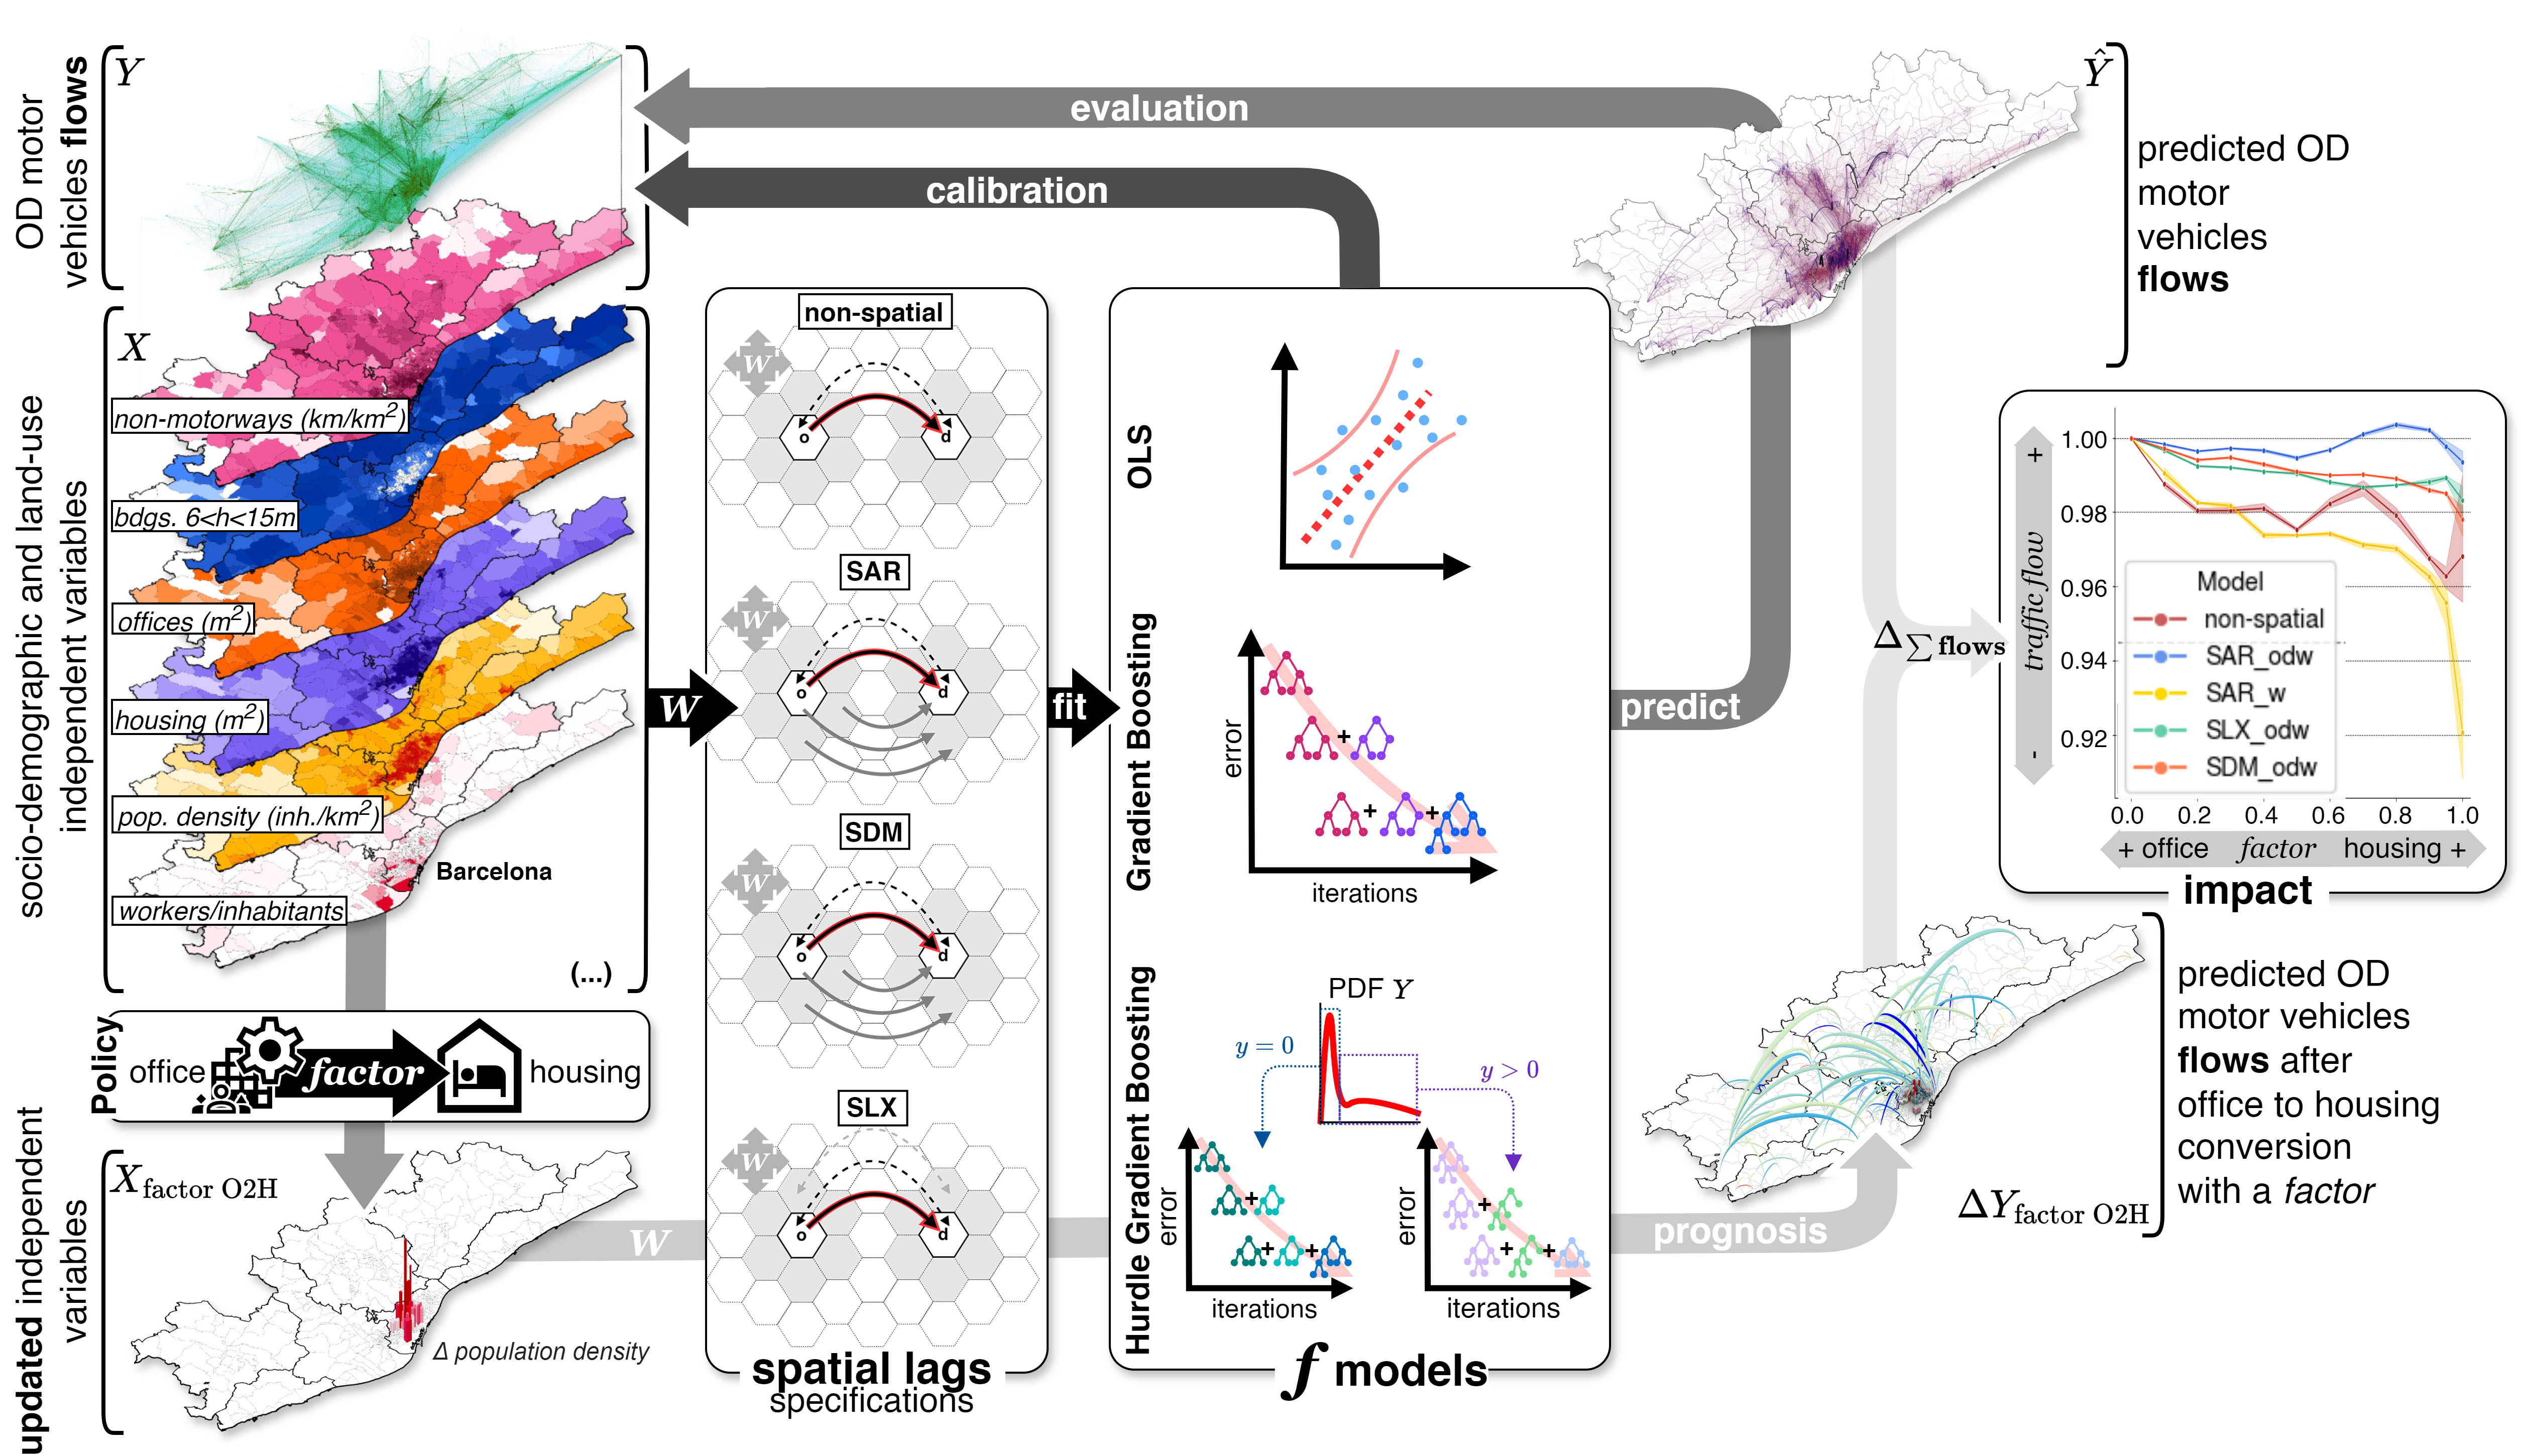
\includegraphics[width=1\textwidth]{graph_abstr.drawio_v5.jpg}
    \caption{Proposed framework. We use socio-demographic, land-use, and topological data to model origin-destination (OD) matrices describing motor vehicle flows between zones in the Metropolitan Region of Barcelona. The Queen adjacency weight matrix (\emph{W}) is used to consider different spatial lag specifications to define spatial econometric models (Spatial autoregressive model --SAR--, spatial Durbin model --SDM--, spatial lags of \emph{X} model --SLX--, and a non-spatial model). Three fitting approaches (Ordinary Least Squares --OLS--, non-parametric gradient boosting, and also a two-part Hurdle model with gradient boosting) are tested and evaluated against the ground truth. Finally, the outperforming two-part Hurdle gradient boosting model is used to test how converting offices into housing impacts overall OD vehicular traffic.}
    \label{fig:graph_abstract}
\end{figure*}

Our article begins with an introductory section where we present a review of the three main components of the research:  spatial (econometric) interaction models in Subsection~\ref{sub:ETRCO2H_1.1intro_spatial_models}, the prediction of OD commuter flows matrices in Subsection~\ref{sub:ETRCO2H_1.2intro_pred_OD}, and the assessment of existing trends in urban planning and city renovation in Subsection~\ref{sub:ETRCO2H_1.3intro_urban}. Then, Section~\ref{sec:ETRCO2H_methods} focuses on technical implementation details, presenting the sources and processing of data, and the statistical learning methods to fit the considered models. Section~\ref{sec:ETRCO2H_results} shows the evaluation of the models and the impact on OD vehicle flows resulting from their application to potential scenarios where office and commercial built-up areas are transformed into residential use in Barcelona. Finally, Section~\ref{sec:ETRCO2H_Discussion} discusses further implications of the use of these models, and Section~\ref{sec:ETRCO2H_Limitations} presents a discussion of limitations and next steps, followed by the concluding remarks in Section~\ref{sec:ETRCO2H_conclusion}.

\subsection{Spatial interaction models}
\label{sub:ETRCO2H_1.1intro_spatial_models}
%gravity vs intervening opportunities

Research in geography trying to find relationships between land use and human mobility has used analogies based on physics \citep{Carey1859PrinciplesScience}.
However, fundamental challenges regarding how to model mobility well persist until today. ``Spatial interaction models" refer to a number of methods that have tried to understand, analyze, model, and predict spatial dynamics. This includes models for flows between origins and destinations, which are applied in a diverse number of fields such as trade, transportation, logistics, retail sales, knowledge exchange, commuting, and human migrations in general \citep{Sen1995GravityBehavior, Margaretic2017SpatialFlows, Thomas-Agnan2021SpatialModels}.

Early attempts to understand the motivations for human mobility can be traced back to migration studies \citep{Ravenstein1885TheMigration}, which tried to identify how the total flows of migrants relate to the size of the locations involved and their distance \citep{Erlander1990TheExtensions}. 
While this approach was extensively used due to its simple interpretability, the limitations of the basic formulation motivated the development of incremental refinements, which led to the so-called ``gravity models" \citep{Zipf1949HumanEffort., Simini2012APatterns}. 
This could be understood from a statistical mechanics perspective as a result of entropy maximization applied to a transportation theoretical problem \citep{Wilson1975SomeReview}.

Gravity models consider spatial information regarding variables that describe the capacity to attract or produce flows. There are ``singly", ``doubly-constrained" or unconstrained models, depending on whether the ``sizes" only of origins, only of destinations, of both of them or none respectively, are considered \citep{Hayes1971SpatialInteraction, Fotheringham1989SpatialApplications, Wilson1975SomeReview}.
This set of spatial interaction models was later extended into a general theory of movement \citep{Alonso1976AMovements, Fotheringham1984FurtherMovement}.  It was also the basis of the first operational land use transport models \citep{Lowry1964AMetropolis}. Despite their limitations (e.g. unreliability, overwhelming complexity) \citep{Lee1973RequiemModels}, these were used in a large number of variations for large-scale urban modeling \citep{Wegener2021Land-UseModels, Iacono2008ModelsTerritory}.

Alternatives such as the ``intervening opportunities model" \citep{Stouffer1940InterveningDistance}, bid-rent theory \citep{Alonso1964LocationRent}, or the random utility maximization models \citep{Block1959RandomResponse} were able to adjust to different types of flows, considering individual behavior, microeconomic theory, and psychological aspects. Such utility-based approaches modeled discrete choice \citep{McFadden1974ConditionalBehavior, Ben-Akiva1985DiscreteDemand} as a function of location features based on behavioral, cognitive, and psychological aspects to overcome the flaws of purely aggregated spatial interactions. 
Eventually, this type of approach was enriched by the perspective of spatial cognition and perception, including spatial structure in the decision process and accounting for people's bounded capacity to process information. This led to ``competing destinations" models \citep{Fotheringham1983ADestinations}, which tried to deal also with the shortcomings of the distance decay as compared to empirical observations.
More recently, the ``radiation model" \citep{Simini2012APatterns} and its extensions, aiming to be more robust with regard to changes in scale \citep{Simini2013HumanApproach, Yang2014LimitsCalibration}, introduced a focus on topological features. In general, this led to a more universal interpretation of flows \citep{Masucci2013GravityFlows} and eventually resulted in a better match with reality, thereby outperforming previous gravity and distance-based models \citep{Noulas2012AMobility}.

These models tried to explain the spatial interactions based on features of the origin and destination zones considered separately, and also metrics reflecting differences between origin and destination. By implicitly considering these features separately and cost-like variables between origin and destinations, they assumed the spatial independence of the observations. However, the observed spatial correlation in residuals of the traditional gravity models \citep{Moran1950NotesPhenomena.,Curry1972AFlows, Griffith1980ExplorationsInteraction.} questioned the assumption of independence between flows and led to the introduction of spatial autocorrelation in the so-called spatial autoregressive models (SAR). To capture these spatial dependences, these models included spatial lags, which means weighted averages of variable values ---in the case of SAR models, the dependent variable, hence the name--- for neighboring locations. Intuitively, these models rely on the observation that large flows between two given areas would be also connected to larger flows between neighboring zones to the given areas as a result of spatial spillovers \citep{LeSage2008SpatialFlows}.

\subsection{Estimation and prediction of OD flow matrices}
\label{sub:ETRCO2H_1.2intro_pred_OD}

In mobility studies and transport planning, the Origin-Destination (OD) matrix is a standard representation of aggregated movement in a certain area between locations over a period of time. It takes the form of a $n \times m$ matrix, where $n$ and $m$ denote the number of `Origin' and `Destination' locations, respectively, with $T_{ij}$ representing travel between locations $i$ and $j$. Typically, these locations can be non-overlapping zones that divide a larger area, and they can be simultaneously origins and destinations, leading to $n = m$. Ultimately, the OD matrix's spatial resolution is limited by the granularity of the available dataset. 

The determination of OD flows is central to urban planning, transportation, mobility, geography, regional economics, and social physics. Within the broad interdisciplinary research using OD matrices, one can distinguish different methods depending on the specific practical task at hand: the temporal forecasting of dynamic flows, the flow estimation based on observations, the bottom-up construction of OD matrices from individual data, and the prediction of flows based on spatial features \citep{Rong2023AnTechniques}, which is the main focus of this research.

Traditional methods to elaborate OD matrices were based on surveys and counts, which required extremely costly processes and resulted in limited samples, therefore affecting precision \citep{Axhausen2002ObservingDiary, Iqbal2014DevelopmentData, Schuessler2009ProcessingInformation}.  Among the bottom-up approaches based on surveys, individual data, and discrete choice approaches, the 4-step method has been widely used in research and practice \citep{McNally2007TheModel, Ortuzar2011ModellingTransport}. Recently, however, information and communication technologies (ICT) have provided a massive amount of human behavioral data \citep{Lenormand2015InfluenceMobility}, and new data-driven methods have been developed to estimate OD matrices directly \citep{Caceres2008ReviewNetworks}.

Modeling OD matrices is particularly challenging due to some features of the dynamics they represent  \citep{Thomas-Agnan2021SpatialModels}:
\begin{enumerate}
    \item They are zero-inflated or sparse, meaning most matrix elements are zero, indicating that many zones have no flows between them.
    \item The main diagonal, which represents intra-zone flows, tends to have much higher values.
    \item Vehicle flows may not follow a pure gravity-like law, meaning that for very short distances they may not be very common.
\end{enumerate}

For completeness, we begin by discussing gravity models. The conventional mathematical approach of this classical spatial interaction model follows Equation~\ref{eq:classical_spatial_interaction_model} \citep{LeSage2010SpatialFlows}:
\begin{equation}\label{eq:classical_spatial_interaction_model}
\mu(i,j) = C\ O(i)\ D(j)\ S(i,j) ,
\end{equation}
where $\mu(i,j)$ represents the expected flow, $C$ is a fit constant, $O(i)$ and $D(j)$ are respectively origin and destination variables, and $S$ is some separation factor between origin and destination. It is common to use ordinary least squares (OLS) with log-transforms on both sides of the equation \citep{Fotheringham1989SpatialApplications, Flowerdew1982ADISTRIBUTION}. This results in the so-called log normal spatial interaction model in Equation~\ref{eq:log_normal_spatial_interaction}:
\begin{equation}\label{eq:log_normal_spatial_interaction}
\log(T_{ij}) = \log(k) + \beta_i \log(O_i) + \beta_d \log(D_j) + \gamma  S_{ij} + \epsilon ,
\end{equation}
where $O_i$ and $D_j$ are vectors of attributes in the origin and destination zones respectively, $S_{ij}$ the vector of some metric of separation (e.g. distance, cost) between origins and destinations, and $k$, $\beta_i$, $\beta_d$ and $\gamma$ are fit parameters to be estimated \citep{Flowerdew1982ADISTRIBUTION}. However, this approach has a few shortcomings: 
\begin{enumerate}
\item flows do not necessarily follow a (log) normal distribution; 
\item homoscedasticity of errors may not apply; and 
\item zero values in the logarithms constitute a problem \citep{Fotheringham1989SpatialApplications}. 
\end{enumerate}

Alternatively, flows between zones have sometimes been assumed to result from a Poisson process \citep{Cameron2013RegressionData}.
However, commuting flows do not necessarily follow a Poisson distribution, which may result in misspecifications of the model \citep{Farmer2011CommutingTravel-to-work}. Furthermore, overdispersion in OD matrices (where variance is greater than the mean) may result from spatial dependencies between flows or the excess of zero values. Therefore, alternative models have been suggested, such as the negative binomial model \citep{Cameron2005Microeconometrics, Hilbe2011NegativeRegression} or quasi- and pseudo-likelihood methods \citep{Farmer2011CommutingTravel-to-work, Jeong2023EstimationApproach}. 
Additionally, Tweedie distributions \citep{Tweedie1984AnFamilies} have been used in actuarial studies to model zero-inflated data, which cannot be transformed to normal distributions \citep{Zhou2020TweedieData}.
More specific strategies to handle an extreme excess of zeroes include the Zero-inflated model \citep{Lambert1992Zero-InflatedManufacturing} and the Hurdle model \citep{Cragg1971SomeGoods, Mullahy1986SpecificationModels}. 
Generally, both approaches (including a negative-binomial regression and a truncated Poisson regression) have shown reliable results \citep{Farmer2011CommutingTravel-to-work}.

Traditional frameworks such as the gravity model, the intervening opportunities model, and the radiation model introduced in the previous subsection have been recently expanded by adding more data from different sources, including land use data \citep{Liu2020HowPerspective}. It was also proposed to combine them, resulting in an increase of predictive power \citep{Rong2023AnTechniques}. Additionally, more sophisticated machine learning models such as Support Vector Regression (SVR) \citep{Rodriguez-Rueda2021OriginDestinationModel} and non-parametric approaches with tree-based algorithms, particularly in the case of Gradient Boosting \citep{Pourebrahim2019TripData, Robinson2018AMigration, Schimohr2023PredictionAlgorithm, Rowe2022AssessingWeather, Ramesh2021Station-levelSystem, Cheng2021Flow-basedCarsharing}, have been shown to often improve traditional methods. 
More recently, the Hurdle model \citep{Cragg1971SomeGoods, Mullahy1986SpecificationModels} has also been used in combination with gradient boosting to improve the modeling and prediction of count data with an excess of zero values, where simpler Poisson regressions have been limited \citep{Krasniqi2022ParametricFrequency, Xu2024GeneralizedDemand}.

When relaxing the independence of flows assumption, there are different ways of specifying how spatial interactions take place between zones: 
\begin{enumerate}
    \item endogenous spatial dependence in the dependent variable (i.e. spatial lags of $Y$);
    \item exogenous spatial dependence across the independent variables (i.e. spatial lags of explanatory variables $X$); and
    \item spatial dependence in the error terms.
\end{enumerate}
Complementarily, spatially dependent interactions $i$ may be considered based on origins ($o$), destinations ($d$), and origin-to-destination relations ($w$).
In the spatial autoregressive models, OLS may lead to unreliable estimations due to the correlation between the endogenous spatial lags and the errors. This has motivated the development of different specifications for the spatial dependence as shown in Figure~\ref{fig:diagram_interactions} and Table~ \ref{tab:spatial_autoregressive_models} (SAR, SEM, SAC) based on restricting parameters of the GNS (General Nesting Spatial) model \citep{Elhorst2014SpatialEconometrics}, which is known as filtering \citep{Anselin1988SpatialModels}. 
Additional estimation approaches have been developed to fit spatially dependent models such as the eigenfunction spatial filtering (ESF) method \citep{Fischer2008ModelingUnion}, the two-stage least squares (2SLS), the generalised method of moments (GMM), the use of instrumental variable estimator (2IV), and the quasi-maximum likelihood (QMLE) \citep{Qu2015EstimatingMatrix, Schatzmann2017SpatialMatrices}. Together with tree-based machine learning statistical methods, they have shown their power to implicitly model spatial interactions \citep{Credit2022SpatialAngeles}.

\begin{figure*}[ht!]
    \centering
    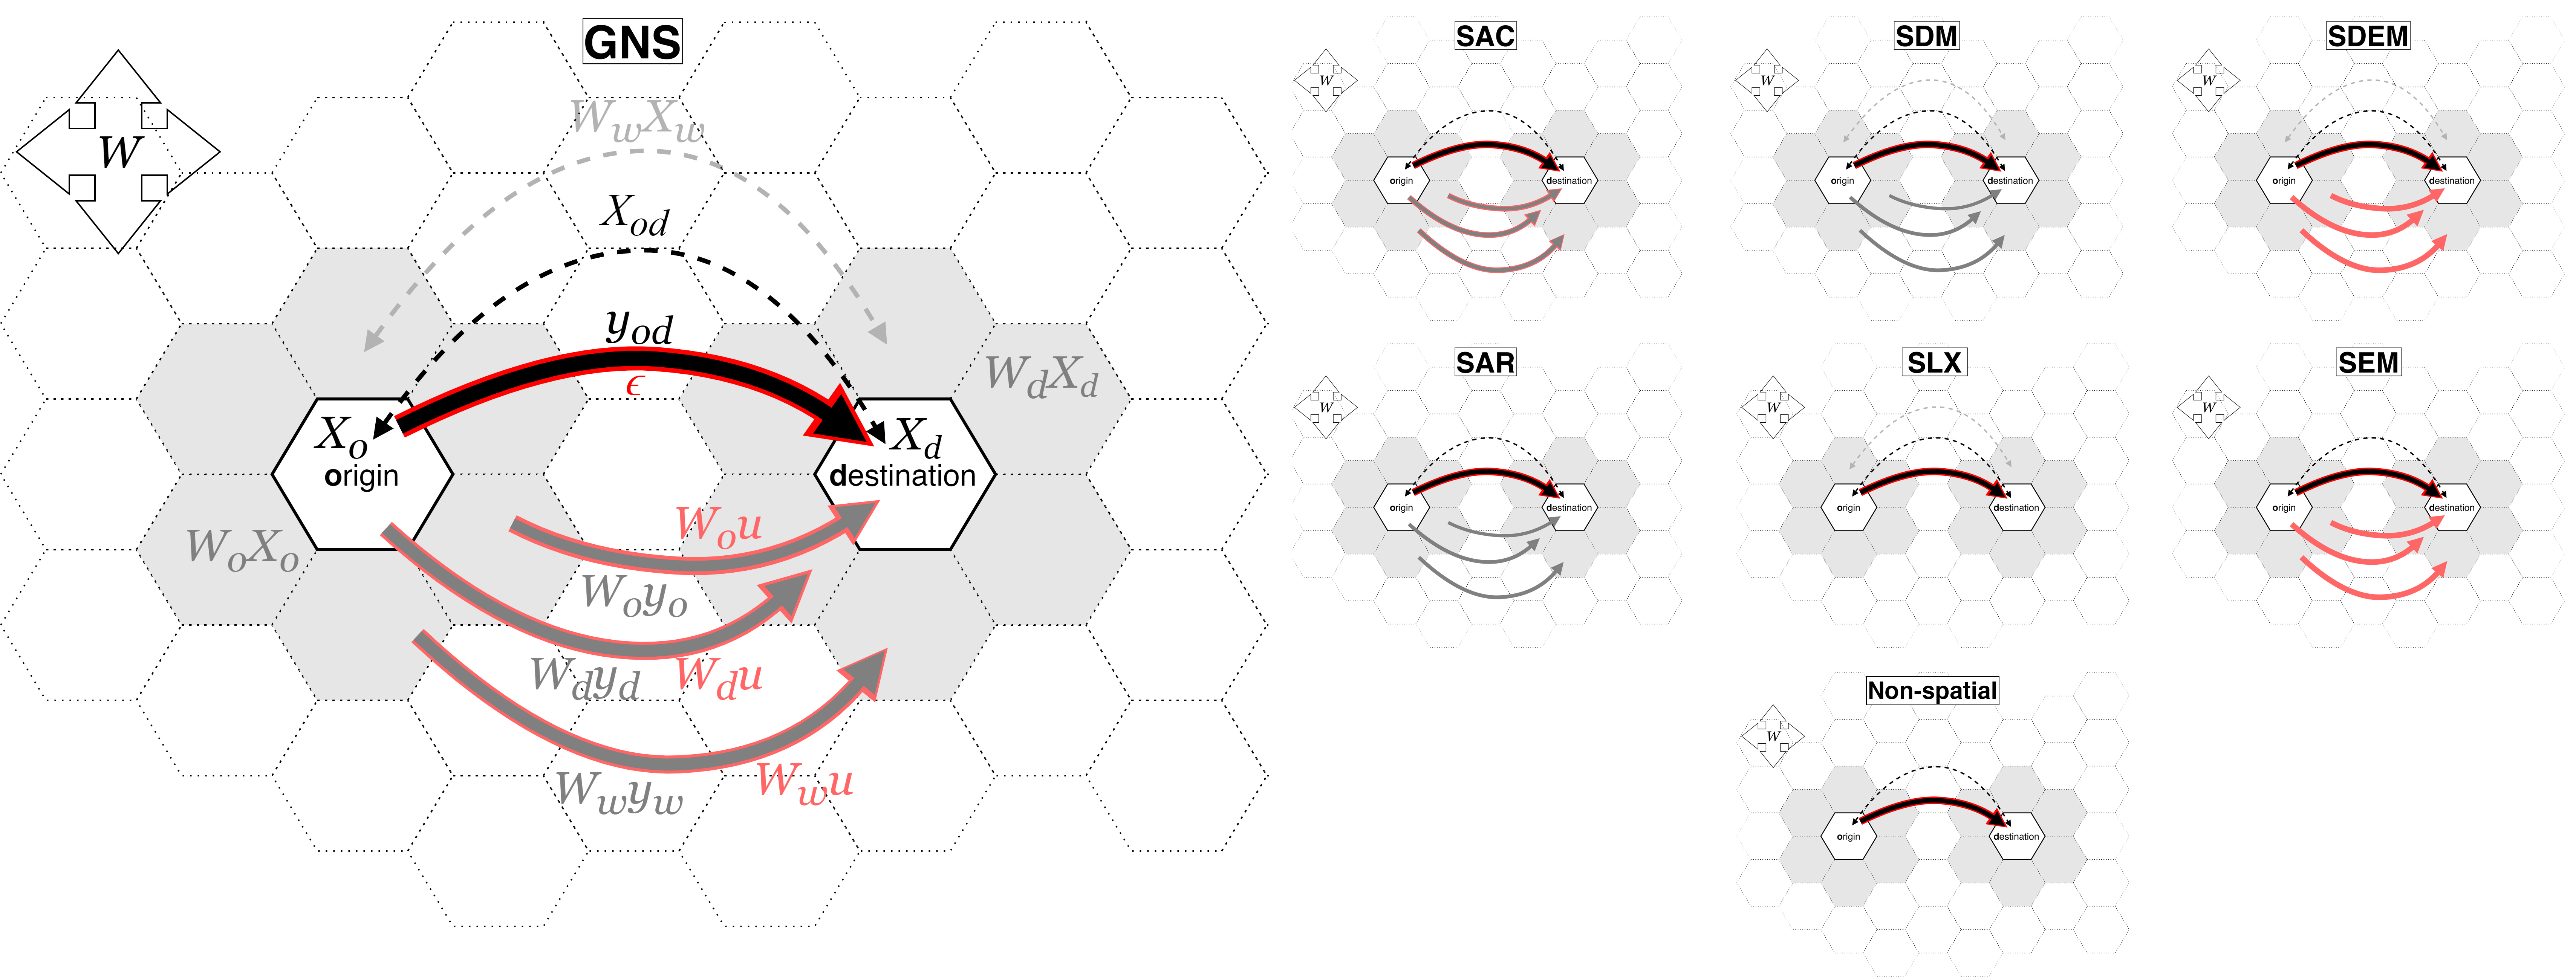
\includegraphics[width=1\textwidth]{diagram_interactions_H_nolabels.jpg}
    \caption{Depiction of Spatial Econometric Models described in Table~ \ref{tab:spatial_autoregressive_models} based on the General Nestin Spatial model (GNS) with all the possible spatial interactions effects between origin and destination zones, including spatially lagged effects from their neighbouring zones highlighted in grey, where $y_{od}$ is the dependent variables (i.e. some commuting flow in this research) between origin and destination, $X_o$ and $X_d$ is a set of explanatory independent variables of the origin and destination respectively, $X_{od}$ a set of distance and difference-based variables between origin and destination, $W$ is a spatial weight matrix based on some adjacency rules between cells, $W_o X_o$ and $W_d X_d$ are exogeneous interaction effects from a set of spatially lagged independent variables $X_o$ and $X_d$ in the neighbouring zones to the origin and destination respectively, $W_w X_w$ a exogenous interactions effects from lagged independent variables resulting from the distance or difference-based variables between neighbouring zones of origin and destination. Error terms are highlighted in red, where $W_o u$ and $W_d u$ are errors due to spatially correlated residuals in the neighboring zones to origin and destination respectively, $W_w u$ are the errors caused by spatially correlated residuals in the distance or difference-based interactions between origin and destination neighboring zones, and $\epsilon$ is the random error term.}
    \label{fig:diagram_interactions}
\end{figure*}

% \usepackage{color}
% \usepackage{tabularray}
\definecolor{Silver}{rgb}{0.752,0.752,0.752}
\begin{table*}[ht!]
\centering
% \captionsetup{labelformat=empty}
\caption{Spatial Econometric Models Specifications generalized for origin-destination flows, adapted from \citep{HalleckVega2015TheModel, Elhorst2014SpatialEconometrics, Margaretic2017SpatialFlows}, with $U = \lambda_i W_i u + \epsilon$ and $i=o,d,w$, where $y$ (dependent variable) is a $N\times1$ vector of flows by stacking the columns of the $n \times m $ OD matrix, $W_iy$ denotes the endogenous interactions effects among the dependent variable $y$, $W_i X_i$ the exogeneous interactions effects among the explanatory variables $X_i$, and $W_i u$ the  interactions effects among the error term. $o,d,w$ refers respectively to the origin, destination, and origin-to-destination spatial dependence. $W_i$ is a nonnegative row-standardized contiguity $n \times m$ matrix describing the spatial structure of the zones, $\alpha \iota_N$ is a $N\times1$  constant parameter vector, $\rho_i$ is the spatial autoregressive coefficient, $\lambda_i$ is the spatial autocorrelation coefficient, and $\beta_i$ and $\theta_i$ are fixed parameter to be estimated  \citep{Elhorst2014SpatialEconometrics, LeSage2008SpatialFlows,Porojan2001TradeRevisited}. The General Nesting Spatial model (GNS) included all possible spatial interactions effects. Spatial filtering by restricting parameters $\rho$, $\theta$ and $\lambda$ generate specific spatial model structures \citep{Jiao2021ForecastingModel, Anselin1988SpatialModels}}
\label{tab:spatial_autoregressive_models} 
\resizebox{\linewidth}{!}{%
\begin{tblr}{
  row{even} = {Silver,c},
  row{3} = {c},
  row{5} = {c},
  cell{1}{1} = {c},
  cell{1}{2} = {c},
  cell{7}{1} = {c},
  cell{7}{2} = {c},
  vline{2-3} = {2,4,6}{white},
  hline{2,4,6} = {-}{},
}
                                                                                                            & {\textbf{GNS~ }General Nesting Spatial Model\\$y = \alpha \iota_N + \rho_i W_i y + X_i \beta_i + W_i X_i \theta + U$} &                                                                                                      \\
no lags of X ($\theta=0$)                                                                                     & no lags in errors $(\lambda=0)$                                                                                       & no lags in y $(\rho=0)$                                                                              \\
{\textbf{SAC} Spatial Autoregressive Combined Model\\$y = \alpha \iota_N + \rho_i W_i y + X_i \beta_i + U$} & {\textbf{SDM} Spatial Durbin Model\\$y = \alpha \iota_N + \rho_i W_i y + X_i \beta_i + W_i X_i \theta + \epsilon$}    & {\textbf{SDEM~ }Spatial Durbin Error Model\\$y = \alpha \iota_N + X_i \beta_i + W_i X_i \theta + U$} \\
no lags in errors $(\lambda=0)$                                                                             & no lags in y $(\rho=0)$                                                                                               & no lags of X$(\theta=0)$                                                                             \\
{\textbf{SAR }Spatial Autoregressive Model\\$y = \alpha \iota_N + \rho_i W_i y + X_i \beta_i + \epsilon$}   & {\textbf{SLX }Spatial lags of X Model\\$y = \alpha \iota_N + X_i \beta_i + W_i X_i \theta + \epsilon$}                 & {\textbf{SEM }Spatial Error Model\\$y = \alpha \iota_N + X_i \beta_i + U$}                           \\
no lags in y $(\rho=0)$                                                                                     & no lags of X $(\theta=0)$                                                                                             & no lags in errors $(\lambda=0)$                                                                      \\
                                                                                                            & {Non-spatial Model\\$y = \alpha \iota_N + X_i \beta_i + \epsilon$}                            &                                                                                                      
\end{tblr}
}
\end{table*}

While further research is required on how to choose the most appropriate model \citep{HalleckVega2015TheModel}, specific procedures have been proposed \citep{Elhorst2014SpatialEconometrics}, including Bayesian approaches \citep{LeSage2014SpatialApproach, LeSage2016AEffects}. One should take into account that the GNS model with full interactions specification, and also other models considering simultaneously spatial interactions between the dependent variables and the error terms (e.g. SAC), tend to be prone to overfitting \citep{Margaretic2017SpatialFlows}.

Last but not least, we would like to mention recent deep-learning methods for OD prediction. Gravity models have been expanded and adapted to these methods, which outperforms OLS approaches \citep{Simini2021AGeneration}. Similarly, deep learning has been used to capture complex spatio-temporal interactions between mobility patterns and urban form \citep{Cai2022SpatialFlow, Koca2021Origin-destinationStudy, Yeghikyan2020LearningNetworks, Liu2020LearningPrediction, Yao2021SpatialNetworks, Yin2022ConvGCN-RF:Effects, Rodriguez-Rueda2021OriginDestinationModel}. While this may produce very accurate fit results, it tends to have quite limited explanatory power. Therefore, one often speaks of ``black-box algorithms".

\subsection{Impact of changes in urban land use}
\label{sub:ETRCO2H_1.3intro_urban}

Building codes, land use regulations, and in general, laws impact building design as well as allocation and use of space. Consequently, they affect also how people choose the location of their home in relation to their daily activities, including work, and how they distribute their resources (i.e. money, time, energy, and cognitive effort) to fulfill daily tasks \citep{Spadon2019ReconstructingIndicators, Simini2012APatterns, Prytherch2012, Levine2019FromPlanning, Jayarajah2018UnderstandingPlanning}. 

A wide body of research examines commuting flows from various perspectives, ranging from individual to aggregated modeling approaches, particularly with regard to location trade-offs between housing and workplaces. It includes the study of differential behaviors across a number of socio-demographic factors such as gender, geographic locations, minorities, or urban structure \citep{Farmer2011CommutingTravel-to-work, Rong2023AnTechniques}.

The impacts of teleworking on the environment and energy consumption have been extensively studied \citep{Giovanis2018, Dissanayake2008, Fu2012EnvironmentalSocio-demographics, Koenig1996UsingProject, Kitou2008ExternalTelework}. However, there is a lack of consensus on whether the outcomes are positive or negative, and spatial implications are often overlooked \citep{Dissanayake2008,Kitou2008ExternalTelework, Bussiere2002Impact1996-2016, Jaff2018EstimatingMalaysia}. While teleworking has been extensively studied across societal, economic, and transportation dimensions, its direct impact on land use in city and territorial planning has not been adequately addressed, yet \citep{Zenkteler2019Home-basedResponse}. This is crucial, however, for the development of policies and building codes. While urban modeling has been used to assess particular policies and planning interventions in cities \citep{Alonso2017ModellingMadrid, Lopane2023AModeling} for a long time, it is increasingly being used as a decision-making tool in urban planning as part of the broader paradigm promoting the use of ``urban digital twins" \citep{Batty2018, Bettencourt2024RecentTwins}.

% teleworking and urban form \citep{Nilles 1991}
Since the COVID-19 pandemic, teleworking has surged, and cities are still dealing with the aftermath of this shock. However, current trends are mixed: On the one hand, companies are trying to balance the teleworking of employees with attempts to keep the vast amount of office space in use (partly to avoid disruptions in the real estate market). On the other hand, in many cities there is a serious shortage of affordable housing \citep{Myers2021}, which causes longer commuting times and social problems, thereby impacting sustainable city development and quality of life. In the meantime, downtown and commercial centers of cities are struggling to recover pre-COVID-19 activity levels, particularly in cases where single-use zones have been promoted \citep{Chapple2023TheCities}. This leads to increasing concerns regarding the future usability and use of commercial and office buildings. In some cities, such buildings are now increasingly refurbished and turned into space for housing \citep{EYStrategyandTransactions2023The2023, AjuntamentdeBarcelona2024, Frei2023a, Schneebeli2021a, Rohwetter, Tagesschau, Bloomberg2021a, Meyer2024a}. However, adaptive reuse of buildings should not considered novel, as it has been a common historical phenomenon in cities \citep{Remy2014}.

Therefore, the development of accessible, transparent, and actionable prognosis tools, which can help to anticipate the effects of planning decisions in cities is a growing field \citep{Batty2018}. However, there are still various challenges to be addressed. Future tools should be able to consider more data and complex interactions while taking into account new theories combining data science and complexity science \citep{Caldarelli2023}. 
Hence, ongoing research aims to offer a quantitative anticipated assessment of the impact of changing use 
%the impact of potential transformations of existing buildings 
of city space and existing buildings, to cope with changing needs and requirements. In particular, this research focuses on which would be the potential impact on mobility, if commercial and office buildings were converted into residential buildings. Studies in the past have been mostly restricted to the economic impact \citep{EYStrategyandTransactions2023The2023, Remy2014}.

\section{Methods}
\label{sec:ETRCO2H_methods}

In the following, we will extend the use of spatial econometric models with gradient boosting to estimate the effect of the transformation of existing commercial and office spaces in Barcelona into housing. 

\subsection{Data}
\label{subsec:ETRCO2H_data}

The geographic scope of our study spans the Metropolitan Region of Barcelona (\emph{Regió Metropolitana de Barcelona} or RMB) which covers 3126 km\textsuperscript{2} with about 5,103,000 inhabitants.

Spatial aggregation plays a crucial role in the analysis of urban phenomena. Different levels of aggregation affect the resulting granularity and distribution of data. A discretization of space is the most frequent approach. 
Specifically, we use the zonal division of the RMB into 577 areas by the IDESCAT (the Catalan Institute of Statistics) for the purpose of transportation planning.
Figure~\ref{fig:data_maps} shows the granularity of the areas:
they are smaller than neighborhoods, wards, or districts, and just slightly bigger than census tracts. 
This spatial aggregation is used as a reference to map and organize the rest of the data. This requires spatial features engineering, either to create new features from source data (e.g. counting points of interest within each zone and creating the spatial lags) or adjust to this zoning aggregation through map matching and area interpolation techniques
\citep{Eicher2001DasymetricEvaluation, Comber2019}. 
%(make figure?).

\begin{figure*}[ht!]
    \centering
    \includegraphics[width=1\textwidth]{fig_maps_data_v01.jpg}
    \caption{Illustration of some of the analyzed data sources: (a) origin-destination flows, (b) population, (c) total built-up area for housing, and (d) total built-up area for offices. The inset displays a zoom into the city center of Barcelona. The limit of the RMB is highlighted as a dashed line.}
    \label{fig:data_maps}
\end{figure*}

Detailed OD flows in the RMB have been obtained from anonymized cell phone tracking data \citep{Calvet2020ObtencioM2019}. Based on a spatio-temporal analysis of the data, in combination with survey and ridership data \citep{PerezSans2021}, it is possible to generate a realistic modal split across the different modes of transportation. The OD estimations for cars have been robustly validated by means of computer simulations at different spatio-temporal scales \citep{ArgotaSanchez-Vaquerizo2021}, and used to assess scenarios of potential urban changes \citep{ArgotaSanchez-Vaquerizo2023LessCity-making}.
Note that, rather than representing daily commuting patterns between homes and activity locations (e.g. work, study, medical care, or shopping), these traffic flows show a more granular picture of trips. This means that what other OD flow matrices may represent as single trips between two locations $i$ and $j$, in our dataset it could be represented as multiple trips in the OD matrix.
All the data refers to the year 2019, to avoid potential distortions by the COVID-19 pandemic in the year 2020 and thereafter.

For the direct analysis and estimation of OD vehicular flows
we considered a combination of land use, socio-demographic, infrastructure, and topological data shown in Tables~\ref{tab:hurdle_ind_vars} and \ref{tab:variable_stats} as potential best explanatory (independent) variables \citep{Krueger2023ACorrections}.
We used step-wise backward elimination in a non-spatial ordinary least squares linear regression approach to select the best explanatory variables among available data. This was combined with the study of the importance levels resulting from XGBoost (Extreme Gradient Boosting) tree-based regression, to eliminate the statistically least significant variables and hence, reduce the over-complexity of the model. 
This is important as the increase in the number of variables can grow very quickly, if origin, destination, origin-destination, and related spatial lags are considered in the model.
As a result, we used diverse data sources: 
\begin{enumerate}
    \item real OD vehicle flows from GPS tracking data; 
    \item socio-demographic data provided by the Spanish National Statistics Institute (INE) and the Statistical Institute of Catalonia (INESCAT); 
    \item land use data, containing building information and urban form features, from the Spanish Cadaster \citep{ MinisteriodeHacienda.GobiernodeEspana2024SedeInicio}, the Global Human Settlement Layer by the European Commission (GHSL) \citep{Pesaresi2023GHS-BUILT-CData}, and Open Street Map (OSM); 
    \item data on infrastructure and transportation facilities as recorded in OSM \citep{OpenStreetMap}; and
    \item topological features regarding the relationship between zones.
 \end{enumerate}
Motivated by the main focus of this research on the shift of urban activities from commercial and office space to residential use, we also preserved the variables related to the land use types in all models, i.e. the total built-up area for residential (\emph{(o/d)\_area\_const\_x\_sum\_V}) and office spaces (\emph{(o/d)\_area\_const\_x\_sum\_O}).

% \usepackage{tabularray}
\begin{table*}
\centering
\caption{Description of the selected independent variables for the Hurdle model and data sources. $(o/d)$ refers to these variables referenced both to origin and destination zones. Otherwise, they are origin-destination relation metrics.}
\label{tab:hurdle_ind_vars}
\resizebox{\linewidth}{!}{%
\begin{tblr}{
  hline{1} = {-}{0.08em},
  hline{2} = {-}{0.05em},
}
\textbf{\textit{Independent variable}}        & \textbf{Description}                                                                                               & \textbf{Source}                         \\
\textit{quickest\_traveltime}                 & {Quickest travel time between the centroid of~\\the origin and destination areas (in seconds).}                    & OSMNX and OSM                           \\
\textit{quickest\_route\_centrality\_mean}    & {Mean of the centrality of the zones crossed by~\\the quickest route between origin and destination.}              & OSMNX and OSM                           \\
\textit{quickest\_route\_centrality\_max}     & {Maximum value of the centrality of the zones crossed\\by the quickest route between origin and destination.}      & OSMNX and OSM.                          \\
\textit{quickest\_route\_centrality\_min}     & {Minimum value of the centrality of the zones crossed~\\by the quickest route between origin and destination.}     & OSMNX and OSM.                          \\
\textit{graph\_degree}                        & Separation degree between origin and destination zones.                                                            & INESCAT                \\
\textit{(o/d)\_pop\_dens\_inh\_per\_km2}      & {Population density in the origin/destination zone~\\(in inhabitants per km\textsuperscript{2}).}                  & INE \\
\textit{(o/d)\_area\_const\_sum\_V}        & {Total built-up surface used for housing in the\\origin/destination zone (in m\textsuperscript{2}).}               & Spanish National Cadaster.              \\
\textit{(o/d)\_area\_const\_sum\_C}        & {Total built-up surface used for retail and commerce in the \\origin/destination zone (in m\textsuperscript{2}).}  & Spanish National Cadaster.              \\
\textit{(o/d)\_area\_const\_sum\_O}        & {Total built-up surface used for offices in the \\origin/destination zone (in m\textsuperscript{2}).}              & Spanish National Cadaster.             \\
\textit{(o/d)\_area\_const\_sum\_E}        & {Total built-up surface used for educational purposes in the \\origin/destination zone (in m\textsuperscript{2}).} & Spanish National Cadaster.              \\
\textit{(o/d)\_area\_const\_sum\_A}        & {Total built-up surface used for parking or storage in the \\origin/destination zone (in m\textsuperscript{2}).}   & Spanish National Cadaster.              \\
\textit{(o/d)\_ratio\_workers}                & {Proportion of workers in the origin/destination zone~\\(workers per inhabitants).}                                & INESCAT                \\
\textit{(o/d)\_len\_non\_motorways\_per\_km2} & {Density of non-motorway roads in the origin/destinationzone~\\(in m/km2)}                                         & OSMNX and OSM.                          \\
\textit{(o/d)\_ratio\_GHSL\_built\_6to15m}    & {Proportion of the origin/destination zone area covered by~\\buildings between 6 and 15 meters tall.}              & GHSL                                    
\end{tblr}
}
\end{table*}
% \usepackage{tabularray}
\begin{table}
\centering
\caption{Description of independent variables. $(o/d)$ refers to these variables referenced both to origin and destination zones. Otherwise, they are origin-destination relation metrics.}
\label{tab:variable_stats}
\resizebox{\linewidth}{!}{%
\begin{tblr}{
  colsep = 0 pt,
  column{even} = {r},
  column{3} = {r},
  column{5} = {r},
  hline{1,17} = {-}{0.08em},
  hline{2} = {-}{},
}
\textbf{\textit{Independent variable}}        & \textbf{mean} & \textbf{median} & \textbf{std} & \textbf{min} & \textbf{max} \\
\textit{daily\_flow}                          & 22.56         & 0.00            & 258.18       & 0.00         & 55560.48     \\
\textit{quickest\_traveltime}                 & 1331.36       & 1211.00         & 789.49       & 0.00         & 5478.00      \\
\textit{quickest\_route\_centrality\_mean}    & 23740.34      & 23618.00        & 9080.83      & 1153.00      & 90793.00     \\
\textit{quickest\_route\_centrality\_max}     & 57538.01      & 50772.00        & 24831.10     & 1153.00      & 90793.00     \\
\textit{quickest\_route\_centrality\_min}     & 3545.38       & 2498.00         & 3286.93      & 324.00       & 90793.00     \\
\textit{(o/d)\_pop\_dens\_inh\_per\_km2}      & 19361.76      & 14270.39        & 19388.50     & 13.03        & 98680.04     \\
\textit{(o/d)\_area\_const\_sum\_V}           & 464649.75     & 364106.00       & 370856.82    & 17462.00     & 3153453.00   \\
\textit{(o/d)\_area\_const\_sum\_C}           & 48990.99      & 36094.00        & 50945.35     & 0.00         & 383410.00    \\
\textit{(o/d)\_area\_const\_sum\_O}           & 32616.09      & 7723.00         & 97394.08     & 0.00         & 1385181.00   \\
\textit{(o/d)\_area\_const\_sum\_E}           & 19558.18      & 12146.00        & 28505.31     & 0.00         & 374419.00    \\
\textit{(o/d)\_area\_const\_sum\_A}           & 66730.56      & 49264.00        & 67618.85     & 0.00         & 825249.00    \\
\textit{(o/d)\_ratio\_workers}                & 0.60          & 0.26            & 2.40         & 0.03         & 53.85        \\
\textit{(o/d)\_len\_non\_motorways\_per\_km2} & 5296.66       & 3328.95         & 5900.24      & 0.00         & 42760.62     \\
\textit{(o/d)\_ratio\_GHSL\_built\_6to15m}    & 0.08          & 0.05            & 0.09         & 0.00         & 0.42         \\
\textit{graph\_degree}                        & 8.82          & 9.00            & 3.80         & 0.00         & 23.00        
\end{tblr}
}
\end{table}

Note that the property data from the Spanish Cadaster \citep{MinisteriodeHacienda.GobiernodeEspana2024SedeInicio} provides very detailed building information such as their location, geometry, footprint, number of properties, type of use, and built surface areas, even in the case of mixed-use multi-story buildings. The individual cadastral records are aggregated per INESCAT zone to provide counts for the total built-up area, number of units, and density for different uses (housing, office, commerce, eateries, cultural, educational, health care and NGOs, religious, and sports facilities). Socio-demographic data from INE are aggregated at the level of census tracts (\emph{secciones censales}, which do not match the INESCAT transportation zones. Therefore, the Python library \emph{Tobler} \citep{Toblercontributors2018ToblerManual} is used to perform areal interpolation using population as ancillary data. OSM data provide counts of amenities, public transit (i.e. bus stops and railway stations) facilities, and the length of the road network.

Separation metrics between zones are based on network and topological features. Instead of the Euclidean distance between the centroids of the zones, the network travel time based on OSM speed data \citep{OpenStreetMap, Boeing2017OSMnx:Networks} is considered more accurate. %\citep{Killer, 2014}. 
The exogenous variable \emph{graph degree} ensures the consideration of topological distances as determinants of human mobility \citep{Simini2012APatterns, Noulas2012AMobility, Ballerini2008InteractionStudy}. This can be connected to a proximity rank, related to the proposed "intervening opportunities" framework \citep{Stouffer1940InterveningDistance}. Complementary, spatial interactions are also captured by introducing other topological metrics, based on graph connectivity built on adjacency, including the separation degree between zones ($graph\_degree$), and centrality statistics of the zones crossed by the quickest routes between zones ($quickest\_route\_centrality\_mean$, $quickest\_route\_centrality\_max$, $quickest\_route\_centrality\_min$).

Data organization and notation follow an origin-centric approach as proposed by \citep{LeSage2008SpatialFlows}. The OD matrix  $T_{n \times m}$ (with $n = m= 577$ being the number of analyzed zones), whose main diagonal represents intra-zone flows, is mapped on a single vector $y_{N \times 1}$ (with $N = n \times m$). The explanatory variables are divided into two sets: (1) a matrix $O_{N \times Q}$ for the origin-specific features resulting from repeating the $q$ explanatory variables of $O_{n \times q}$ \emph{n times}, using $O_{N \times Q} = O_{n \times q} \otimes \iota_n$, where $\iota_n$ is a vector of ones, (2) a matrix $D_{N \times R}$ for the destination-specific features resulting from repeating the $r$ explanatory variables of $D_{m \times r}$ \emph{m times}, using $D_{N \times R} = D_{m \times r} \otimes \iota_m$. Finally, the $p$ separation variables between origin and destinations are transformed similarly to the OD flows, by mapping each of the $S_{n \times m}^{(p)}$ distance matrices on $s_{N \times 1}^{(p)}$ vectors.

To include spillover effects, a first-order queen adjacency based on common edges and corners is used to compute the spatial weight matrix $W$ needed for the spatial lags. Then, it is row-standardized (sum of row elements is 1) to not overweight zones with many neighbors \citep{Griffith2020SomeModels}.
After this, it is possible to derive the spatial dependencies centered in origin, destination, and origin-destination interactions, respectively, as $W_o = I_n \otimes W$,  $W_d = W \otimes I_n$, and $W_w = W \otimes W$ \citep{LeSage2008SpatialFlows}. This allows us to average the neighboring features, flows, or separation metrics, depending on the specification of the spatial econometric interaction model used (Table~\ref{tab:spatial_autoregressive_models}).

\subsection{Modelling}
\label{subsec:ETRCO2H_modelling}

We propose to apply a two-part Hurdle model \citep{Mullahy1986SpecificationModels} based on a non-parametric statistical learning approach using gradient tree boosting \citep{Friedman2001GreedyMachine.}, specifically XGBoost (XGB or Extreme Gradient Boosting) \citep{Chen2016XGBoost:System}. The two-part model first estimates the probability of the dependent variable to be 0 with an XGBoost logistic regression model for the zero-inflated part. Then, it uses an XGBoost truncated Tweedie model \citep{Valero2012ExtendedModel} for the rest of the data. Overall, the selection of this modeling approach is motivated by:
\begin{enumerate}
    \item the high number of zeros, 
    \item the overdispersion of the flows (dependent variable), 
    \item the lack of theoretical and empirical foundations to make conventional assumptions regarding the distribution of data, and 
    \item the complexity of the interactions between the different variables.
\end{enumerate}

XGBoost is an ensemble algorithm rooted in gradient boosting, which employs decision trees iteratively as weak learners to minimize prediction errors \citep{Chen2016XGBoost:System}. 
Weak learners are simple models that perform slightly better than random guessing, such as shallow decision trees. Gradient boosting combines these weak learners sequentially, focusing on minimizing the loss function by learning from the residuals of the previous model, gradually improving prediction accuracy. Designed for scalability and computational efficiency, it stands out for its ability to handle large datasets and learn non-linearities as well as complex and higher-order interactions with minimal training time and without requiring strict assumptions on data distribution.
%, which may turn into unfeasible in real data. 
Through gradient descent, it continuously improves model performance by adding trees in an additive manner, balancing model complexity with regularization techniques like shrinkage and column subsampling to mitigate overfitting. Its versatility extends to various regression tasks, such as Poisson and Tweedie regression. The implementation is supported by Python through the XGBoost package \citep{XGBoostcontributors2022XGBoostDocumentation}. Optimizing both, model structure and hyperparameters, XGBoost has emerged as a highly effective off-the-shelf tool for data mining and is widely used in machine learning competitions and practical applications alike.

For the sake of performance assessment, we also compare the proposed two-part model with one-part, simpler approaches: a parametric OLS regression and a non-parametric Tweedie XGBoost regression. For these three modeling methods, we compare four main treatments for spatial dependence among the ones specified in Table~\ref{tab:spatial_autoregressive_models}: 
\begin{enumerate}
    \item A spatially independent model without spatial interaction terms.
    \item An autoregressive (SAR) model with spatial interaction terms for the dependent variable $Y$ based on origins ($i=o$), based on destinations ($i=d$), based on origin-destination relations ($i=w$), and the three altogether ($i=o,d,w$).
    \item A model with spatial lags of independent variables $X$ (SLX), including the specifications for all interactions ($i=o,d,w$), and only origin and destination-based interactions ($i=o,d$). 
    \item A spatial Durbin model (SDM) including all interactions ($i=o,d,w$).
\end{enumerate}
Our data was divided between training and test datasets with an 80-20 proportion. Additionally, we tuned the hyperparameters of the XGBoost-based model, using Optuna with 5-fold cross-validation during training \citep{Akiba2019Optuna:Framework, Krasniqi2022ParametricFrequency}. 

Furthermore, the level of interpretability and transparency of the models is crucial for the selection and evaluation of the most appropriate model \citep{Huang2023IncreasingExplanations}. To assess this, we used bootstrapping simulation ($n=1000$) to compute the distribution of model metrics in an empirically informed way \citep{DiCiccio1996BootstrapIntervals}. This allowed us to statistically compare their differences in performance, using a non-parametric two-sided Mann-Whitney-U test \citep{Mann1947} (see Figures~\ref{fig:MWU_test_2x2_pvalues} and \ref{fig:MWU_test_2x2_effectSize} in Appendix). To interpret the impact of explanatory variables in the models, we used \emph{Shapley Additive exPlanations} (SHAP) \citep{Lundberg2017APredictions}. This method applies a game theoretical approach \citep{Strumbelj2014ExplainingContributions} to provide robust and consistent feature-importance attributions for each explanatory variable, which is in fact theoretically proven as being the unique solution \citep{Fujimoto2006AxiomaticIndices}.

Whereas non-parametric models do not require one to make assumptions about the distribution of data and about uncertainties regarding the real distributions of the considered data (e.g. commuting flows) \citep{Farmer2011CommutingTravel-to-work}, we decided for a log transform for the explanatory variables, with the standard treatment of adding a constant to deal with zero values. Alternatively, and to avoid bias in the predictions due to the back-transformation, a square root transform was used as the dependent variable, allowing us to simultaneously deal with the case of many zero values. Overall, this data transformation approach turned out to have better performance among other considered alternatives, including Box-Cox and Yeo-Johnson.

\subsection{Accuracy metrics}
\label{subsec:ETRCO2H_accuracy_metrics}

We assess the goodness-of-fit of the considered models with a focus on prediction. Hence we evaluate the models, which were calibrated with the training dataset, out-of-sample (i.e. with unseen data), %from the test dataset 
using five metrics that focus on different types of disagreements between the model and ground truth (Equations~\ref{eq:MAE} to \ref{eq:SQV}). This includes: 

the Mean Absolute Error (MAE)
\begin{equation}
\label{eq:MAE}
MAE(y,\hat{y}) = \frac{1}{n}\sum_{i,j=1}^{n}|y_{ij} - \hat{y}_{ij}|,
\end{equation}
the Root Mean Squared Error (RMSE)
\begin{equation}
\label{eq:RMSE}
RMSE(y,\hat{y}) = \sqrt{\frac{1}{n}\sum_{i,j=1}^{n}(y_{ij} - \hat{y}_{ij})^2},
\end{equation}
the Common Part of Commuters (CPC) 
\begin{equation}
\label{eq:CPC}
CPC=\frac {2\sum_{i,j}^n {\min (y_{ij},\hat{y}_{ij})} }{\sum_{i,j}^n {y_{ij}} +\sum_{i,j}^n {\hat{y}_{ij}}},
\end{equation}
and the Common Part of Links (CPL) 
\begin{equation}
\label{eq:CPL}
CPL=\frac{2\sum_{i,j=1}^{n} 1_{y_{ij} > 0}\cdot 1_{\hat{y}_{ij} > 0}}{\sum_{i,j=1}^{n}1_{y_{ij} > 0}+\sum_{i,j=1}^{n}1_{\hat{y}_{ij} > 0}} .
\end{equation}
Here, $y_{ij}$ represents the number of commuters traveling from origin $i$ to destination $j$ in the observed data (i.e. ground truth),  $\hat{y}_{ij}$ represents the number of commuters traveling from origin $i$ to destination $j$ in the predicted data, and the summation is performed over all origin-destination pairs. 

To measure the deviation of the prediction, we consider MAE and RMSE due to the high dispersion of the OD flow values. MAE is more robust to outliers and is not as much affected by large errors as RMSE, which is nevertheless provided due to the downward bias of MAE \citep{Yeghikyan2020LearningNetworks}. CPC is a common metric to assess the general match of simulated OD values with the ground truth \citep{Lenormand2012ANetworks}, based on the Sorensen index \citep{Sorensen1948AContent}. It ranges from 0, corresponding to no match, to 1, corresponding to a perfect match, and represents the percentage of correctly simulated OD pairs. Additionally, CPL provides a general indication of the topological match between the observed and predicted OD pairs \citep{Lenormand2016SystematicModels}, where $1_A$ is equal to one if the condition $A$ is fulfilled and zero otherwise, resulting in a range between 0, in case of no common links, and 1, in case of complete topological equivalence. 

Finally, we also included the Scalable Quality Value (SQV) 
\begin{equation}
\label{eq:SQV}
SQV = \frac{1}{1 + \sqrt{\frac{{(\hat{y}_{ij} - y_{ij})^2}}{{f \cdot y_{ij}}}}}
\end{equation}
to compare the predicted $\hat{y}_{ij}$ with the ground truth $y_{ij}$ individually between $i$ and $j$. This metric improves the GEH (Geoffrey E. Havers) statistic \citep{Dowling2004TrafficSoftware} and introduces a scaling factor $f$ that depends on the magnitude of the flows to be evaluated (with $f=10000$ in this case for daily flows) \citep{Friedrich2019ScalableValidation}. To handle $y_{ij}=0$ in the numerator, ground truth with zero values is replaced by 0.1. While this metric is mostly used for traffic microsimulation studies, it also allows to leverage different error tolerances, which depend on the magnitude of the flows compared, given the dispersed and extremely skewed distribution (see Table \ref{tab:variable_stats}).

\section{Results}
\label{sec:ETRCO2H_results}
\subsection{Models evaluation}

Table~\ref{tab:all_model_stats} and Figure~\ref{fig:boxplots_results} show the results of the considered models with different specifications for the spatial interactions as described in Table~\ref{tab:spatial_autoregressive_models}. We proposed a two-part Hurdle model \citep{Mullahy1986SpecificationModels} using gradient boosting \citep{Friedman2001GreedyMachine.} with XGBoost \citep{Chen2016XGBoost:System} for modeling the motor vehicle OD flows. We compare this approach with simpler one-part models: a parametric OLS regression and a non-parametric Tweedie regression using also XGBoost (\textit{XGB Tweedie}).
Overall, the two-part Hurdle XGB model outperforms the simpler modeling approaches Ordinary Least Squares (OLS) and XGBoost Tweedie \citep{Chen2016XGBoost:System,Krasniqi2022ParametricFrequency} (Subsection \ref{subsec:ETRCO2H_modelling}) for the considered evaluation metrics (Mean Absolute Error -- MAE, Root Mean Squares Error -- RMSE, Common Part of Commuters -- CPC, Common Part of Links -- CPL, and Scalable Quality Value -- SQV) (Subsection~\ref{subsec:ETRCO2H_accuracy_metrics}). In general, the two-part Hurdle XGB model features higher accuracy, has smaller errors, i.e. lower MAE and RMSE values, and matches the OD flow structure better, i.e. higher CPC and CPL values, independently of the spatial lag specification: MAE values around 6, RMSE around 100, CPC around 0.85 and CPL more sparsely distributed between 0.72 and 0.75. Comparatively, the one-part models feature MAE values around 20, RMSE ranging between 200 and 250, CPC below 0.5, and CPL between 0.41 and 0.42.

% \usepackage{tabularray}
\begin{table*}[h!]
\centering
\caption{Mean values (and standard deviations) of accuracy metrics for the analyzed models from bootstrapping simulation ($n=1000$). SQV values refers to the percentage of $ij$ pairs whose SQV value is larger than 0.85, which is considered the minimum threshold to be considered a good match \citep{Friedrich2019ScalableValidation}. For full statistical details see Tables~\ref{tab:append_results_ols_SHP} to \ref{tab:append_results_2part_hurdle_SHP} in \ref{sec:appendix}.}
\label{tab:all_model_stats}
\resizebox{\linewidth}{!}{%
\begin{tblr}{
  colsep=1pt,
  column{6} = {r},
  column{9} = {r},
  column{12} = {r},
  column{15} = {r},
  column{18} = {r},
  column{21} = {r},
  column{24} = {r},
  cell{1}{1} = {r=2}{},
  cell{1}{3} = {c=2}{c},
  cell{1}{5} = {c},
  cell{1}{6} = {c=11}{c},
  cell{1}{17} = {c},
  cell{1}{18} = {c=5}{c},
  cell{1}{23} = {c},
  cell{1}{24} = {c=2}{c},
  cell{2}{2} = {r},
  cell{2}{6} = {c=2}{c},
  cell{2}{8} = {c},
  cell{2}{9} = {c=2}{c},
  cell{2}{11} = {c},
  cell{2}{12} = {c=2}{c},
  cell{2}{14} = {c},
  cell{2}{15} = {c=2}{c},
  cell{2}{17} = {c},
  cell{2}{18} = {c=2}{c},
  cell{2}{20} = {c},
  cell{2}{21} = {c=2}{c},
  cell{2}{23} = {c},
  cell{2}{24} = {c=2}{c},
  cell{3}{1} = {r=5}{},
  cell{3}{3} = {r},
  cell{4}{3} = {r},
  cell{5}{3} = {r},
  cell{6}{3} = {r},
  cell{7}{3} = {r},
  cell{8}{1} = {r=5}{},
  cell{8}{3} = {r},
  cell{9}{3} = {r},
  cell{10}{3} = {r},
  cell{11}{3} = {r},
  cell{12}{3} = {r},
  cell{13}{1} = {r=5}{},
  cell{13}{3} = {r},
  cell{14}{3} = {r},
  cell{15}{3} = {r},
  cell{16}{3} = {r},
  cell{17}{3} = {r},
  hline{1,18} = {-}{0.08em},
  hline{2} = {3-4,6-16,18-22,24-25}{},
  hline{3} = {2-4,6-7,9-10,12-13,15-16,18-19,21-22,24-25}{},
  hline{8,13} = {-}{},
}
\textbf{model}                                                           & \textbf{spatial interaction} & \textbf{non-spatial} &           &  & \textbf{SAR}   &           &  &            &           &  &            &           &  &            &           &  & \textbf{SLX}   &           &  &              &           &  & \textbf{SDM}   &           \\
                                                                         & \textit{filtering}           &                      &           &  & \textit{o,d,w} &           &  & \textit{o} &           &  & \textit{d} &           &  & \textit{w} &           &  & \textit{o,d,w} &           &  & \textit{o,d} &           &  & \textit{o,d,w} &           \\
\textbf{OLS}                                                             & MAE                          & 22.551               & (±0.933)  &  & 20.175         & (±0.866)  &  & 20.313     & (±0.869)  &  & 21.370     & (±0.897)  &  & 21.095     & (±0.892)  &  & 22.363         & (±0.922)  &  & 22.411       & (±0.923)  &  & 19.893         & (±0.864)  \\
                                                                         & RMSE                         & 237.275              & (±37.749) &  & 224.204        & (±39.301) &  & 224.850    & (±39.163) &  & 232.005    & (±38.515) &  & 229.991    & (±38.794) &  & 237.576        & (±37.794) &  & 237.692      & (±37.779) &  & 223.777        & (±39.393) \\
                                                                         & SQV (\%0.85)                 & 85.269               & (±0.141)  &  & 92.843         & (±0.101)  &  & 92.964     & (±0.101)  &  & 91.090     & (±0.112)  &  & 90.832     & (±0.116)  &  & 86.301         & (±0.140)  &  & 85.617       & (±0.143)  &  & 93.441         & (±0.095)  \\
                                                                         & CPC                          & 0.241                & (±0.008)  &  & 0.416          & (±0.010)  &  & 0.411      & (±0.010)  &  & 0.329      & (±0.009)  &  & 0.354      & (±0.009)  &  & 0.253          & (±0.009)  &  & 0.250        & (±0.008)  &  & 0.429          & (±0.010)  \\
                                                                         & CPL                          & 0.415                & (±0.002)  &  & 0.415          & (±0.002)  &  & 0.415      & (±0.002)  &  & 0.415      & (±0.002)  &  & 0.415      & (±0.002)  &  & 0.415          & (±0.002)  &  & 0.415        & (±0.002)  &  & 0.415          & (±0.002)  \\
{\textbf{XGBoost~}\\\textbf{Tweedie}}                                    & MAE                          & 21.667               & (±1.052)  &  & 18.316         & (±0.911)  &  & 19.076     & (±0.960)  &  & 19.790     & (±0.984)  &  & 18.996     & (±0.869)  &  & 20.372         & (±1.004)  &  & 21.371       & (±1.055)  &  & 18.502         & (±0.942)  \\
                                                                         & RMSE                         & 265.009              & (±37.343) &  & 233.223        & (±39.762) &  & 241.709    & (±38.777) &  & 247.254    & (±38.459) &  & 230.342    & (±37.892) &  & 256.271        & (±39.919) &  & 268.537      & (±37.394) &  & 240.452        & (±39.983) \\
                                                                         & SQV (\%0.85)                 & 97.377               & (±0.060)  &  & 97.761         & (±0.056)  &  & 97.612     & (±0.061)  &  & 97.580     & (±0.059)  &  & 97.554     & (±0.059)  &  & 97.760         & (±0.055)  &  & 97.585       & (±0.058)  &  & 97.941         & (±0.053)  \\
                                                                         & CPC                          & 0.406                & (±0.012)  &  & 0.486          & (±0.013)  &  & 0.477      & (±0.013)  &  & 0.453      & (±0.013)  &  & 0.461      & (±0.012)  &  & 0.438          & (±0.013)  &  & 0.425        & (±0.012)  &  & 0.475          & (±0.014)  \\
                                                                         & CPL                          & 0.415                & (±0.002)  &  & 0.415          & (±0.002)  &  & 0.415      & (±0.002)  &  & 0.415      & (±0.002)  &  & 0.415      & (±0.002)  &  & 0.415          & (±0.002)  &  & 0.415        & (±0.002)  &  & 0.415          & (±0.002)  \\
{\textbf{two-part}\\\textbf{XGBoost }\\\textbf{Hurdle }\\\textbf{Model}} & MAE                          & 6.732                & (±0.431)  &  & 6.012          & (±0.377)  &  & 6.182      & (±0.409)  &  & 6.044      & (±0.337)  &  & 6.453      & (±0.408)  &  & 6.109          & (±0.388)  &  & 6.143        & (±0.388)  &  & 5.769          & (±0.382)  \\
                                                                         & RMSE                         & 109.106              & (±18.235) &  & 96.642         & (±17.598) &  & 105.149    & (±18.388) &  & 85.596     & (±16.459) &  & 105.030    & (±18.119) &  & 98.774         & (±18.026) &  & 97.015       & (±18.290) &  & 97.196         & (±17.217) \\
                                                                         & SQV (\%0.85)                 & 96.649               & (±0.068)  &  & 96.436         & (±0.071)  &  & 96.409     & (±0.072)  &  & 96.673     & (±0.069)  &  & 96.376     & (±0.072)  &  & 96.829         & (±0.070)  &  & 96.908       & (±0.068)  &  & 96.658         & (±0.069)  \\
                                                                         & CPC                          & 0.838                & (±0.010)  &  & 0.861          & (±0.009)  &  & 0.858      & (±0.009)  &  & 0.857      & (±0.009)  &  & 0.849      & (±0.010)  &  & 0.856          & (±0.009)  &  & 0.854        & (±0.009)  &  & 0.867          & (±0.009)  \\
                                                                         & CPL                          & 0.723                & (±0.003)  &  & 0.747          & (±0.003)  &  & 0.747      & (±0.003)  &  & 0.726      & (±0.003)  &  & 0.736      & (±0.003)  &  & 0.738          & (±0.003)  &  & 0.734        & (±0.003)  &  & 0.752          & (±0.003)  
\end{tblr}
}
\end{table*}

\begin{figure*}[ht!]
    \centering
    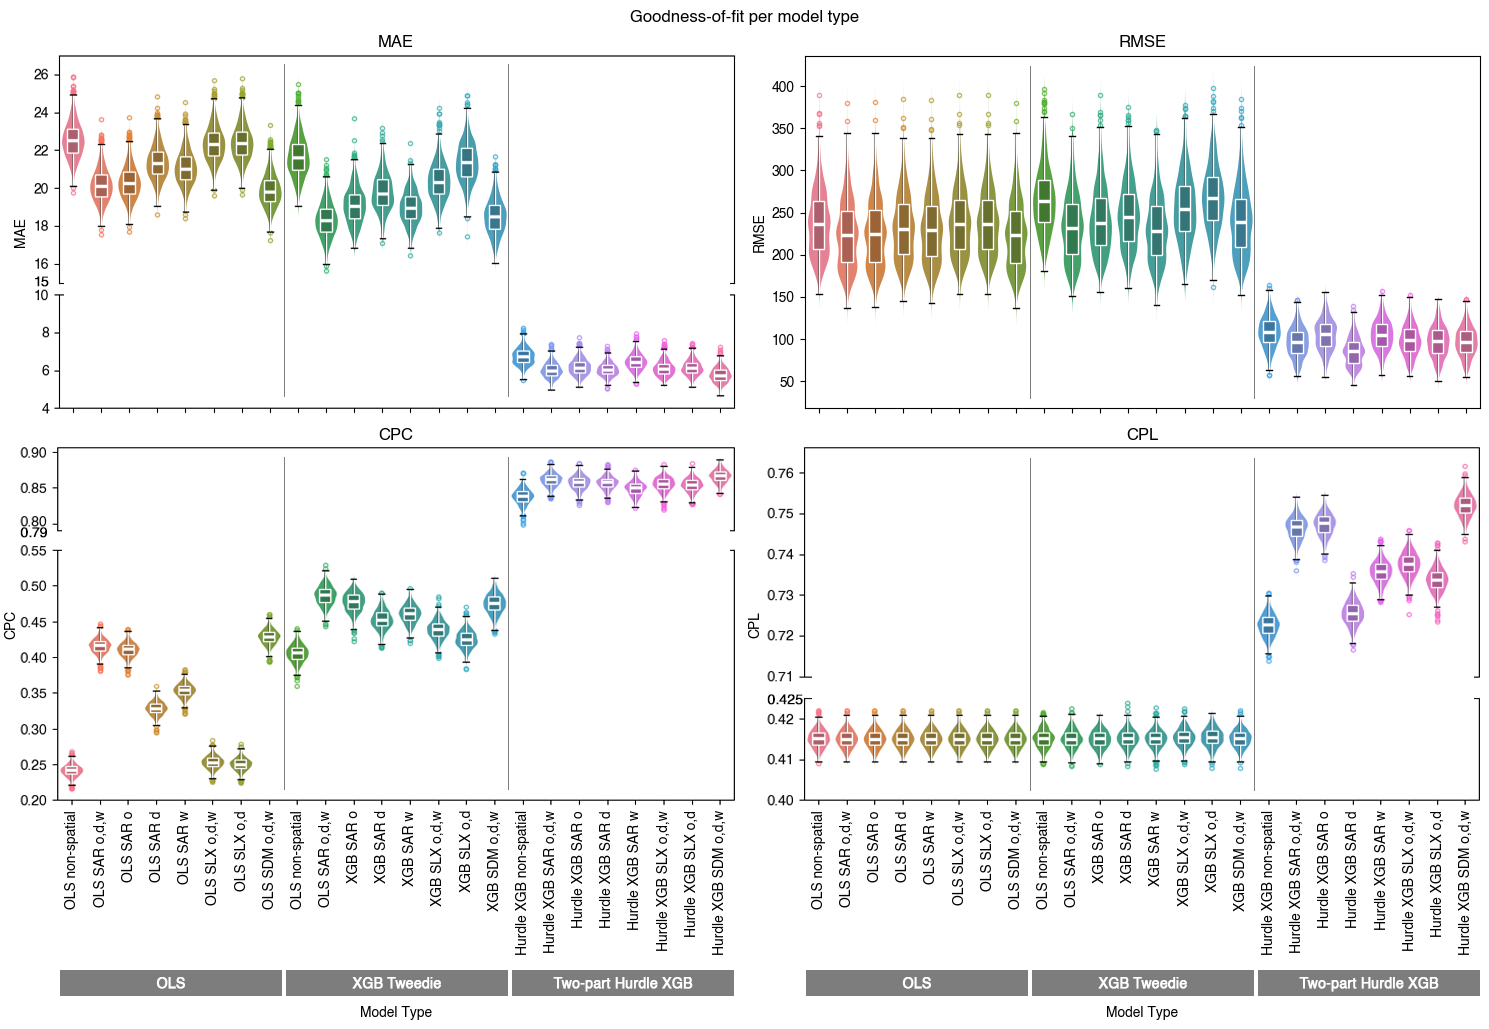
\includegraphics[width=1\textwidth]{fig_all_models_goodness_of_fit_2x2_n1000.png}
    \caption{Goodness-of-fit of the analyzed models from bootstrapping simulation ($n=1000$). The two-part model outperforms the simpler one-part models. Medians are indicated with a thick white horizontal line. Lower MAE and RMSE values and values of CPC and CPL closer to 1 represent better matching with the ground truth.}
    \label{fig:boxplots_results}
\end{figure*}

The main statistically significant ($p{\text -}value<0.05$) differences between model metrics according to the Mann-Whitney-U test \citep{Mann1947} are observed between the two-part Hurdle XGB model and the one-part OLS and XGB Tweedie models, as shown in Figures~\ref{fig:MWU_test_2x2_pvalues} and \ref{fig:MWU_test_2x2_effectSize} in Appendix.
Different spatial lag specifications within the same modeling approach cause smaller differences. 
Particularly, the one-part models OLS and XGB Tweedie show more similarity across spatial lag specification for MAE, RMSE, and particularly CPL.
Focusing on the two-part Hurdle XGB model, MAE values are very similar. $\text{SAR}_{i=o,d,w}$ and $\text{SAR}_{i=d}$ show slightly lower values ($6.012(\pm0.377)$, $6.044(\pm0.337)$) than $\text{SLX}_{i=o,d,w}$ and $\text{SLX}_{i=o,d}$ ($6.109(\pm0.388)$, $6.143(\pm0.388)$). However, $\text{SDM}_{i=o,d,w}$ shows the lowest MAE value with $5.769(\pm0.382)$.
The RMSE results for $\text{SAR}_{i=o,d,w}$, $\text{SLX}_{i=o,d,w}$, $\text{SLX}_{i=o,d}$ and $\text{SDM}_{i=o,d,w}$ perform similarly and do not show statically significant differences, although the lowest value for this metric is obtained by $\text{SAR}_{i=d}$ with $85.596(\pm16.459)$. Regarding CPC, all the spatial lag specifications for the two-part XGB Hurdle model are statistically different. While $\text{SDM}_{i=o,d,w}$ shows the highest value ($0.867(\pm0.009)$), the other specifications perform very similarly in the range of $0.849-0.858$. The results of CPL are similar with even bigger differences between spatial lag specifications. $\text{SDM}_{i=o,d,w}$ outperforms all others followed by $\text{SAR}_{i=o,d,w}$, $\text{SAR}_{i=o}$.

Overall, the $\text{SAR}_{i=o,d,w}$, $\text{SAR}_{i=o}$, and $\text{SDM}_{i=o,d,w}$ specifications show a slightly better match with ground truth. However, the two-part Hurdle XGB $\text{SLX}_{i=o,d,w}$ model is competitive with other spatial lag specifications, with small differences and without the cost of interaction over-specification as in $\text{SAR}_{i=o,d,w}$ and $\text{SDM}_{i=o,d,w}$ \citep{Griffith2020SomeModels}. 
Furthermore, SLX outperforms all metrics when compared with the non-spatial model. Additionally, when analyzed at the disaggregated level of the individual OD pairs, as shown in Figure~\ref{fig:Hurdle_SLX_matrices}, this model shows a good match with the ground truth, without any apparent spatial structure in the errors and low disagreement based on the modified SQV metric.

\begin{figure*}[h!]
    \centering
    \includegraphics[width=1\textwidth]{figure_mats_2x4.png}
    \caption{Errors of OD matrices for different models between ground truth and predicted values. The top row shows the percentage error. The bottom row shows the accuracy based on the SQV metric. The selected spatial interaction models do not exhibit differences in the error when analyzed at the disaggregated level of OD pairs. The $X$-axis and $Y$-axis show the 577 zones used as OD pairs, grouped in the 7 counties of the RMB.}
    \label{fig:Hurdle_SLX_matrices}
\end{figure*}

The analysis of the SHAP values \citep{Lundberg2017APredictions} among the best-performing spatial interaction specifications of the two-part Hurdle XGB model (Figure~\ref{fig:SHAP}) allows us to better understand the trade-offs %between them 
and the impact of the variables. As a result it is possible to identify the importance of the main distance metric (\emph{quickest\_traveltime}), which is aligned with the main theoretical frameworks used to model flows and exchange between locations. However, the final impact depends on the interplay of other variables. Autoregressive terms (i.e. spatial lags of $Y$) in SAR and SDM tend to have a very high impact when included in SAR and SDM models. Particularly the origin-centric spatial lag of $Y$ (\emph{W\_o\_daily\_flow}) shows a much larger contribution than lags of $Y$ based on destination (\emph{W\_d\_daily\_flow}) or origin-destination (\emph{W\_w\_daily\_flow}) relations. When autoregressive variables are not included, such as in the SLX model, there is an important increase in the contribution of (\emph{quickest\_traveltime}) and topology-related distance metrics (i.e. \emph{graph\_degree}). Also, the centrality measure  (\emph{quickest\_route\_centrality\_max}) of the quickest paths, which is a variable relating to quickest and topological distances, indicates the importance of the position of the zones along the most frequent quickest routing paths and how they may relate to the counting of vehicle trips.

\begin{figure*}[ht!]
    \centering
    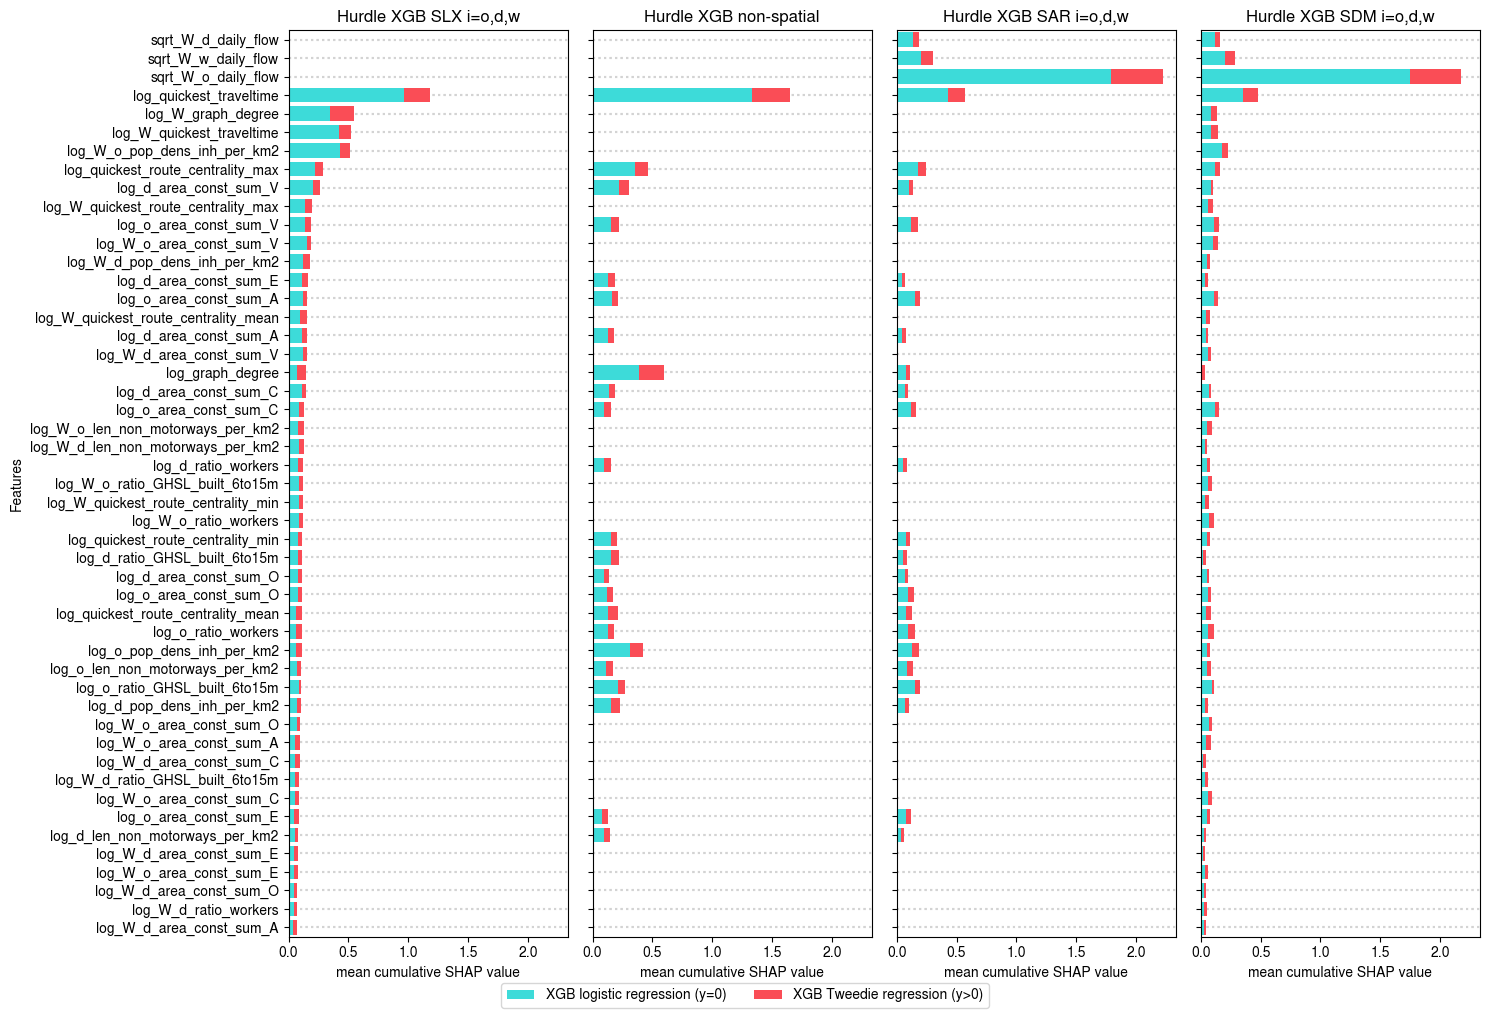
\includegraphics[width=1\textwidth]{fig_SHAP_importances_4models_SDM.png}
    \caption{Summary of the cumulative average impact on the magnitude of the model output, separately for each explanatory variable, using SHAP values \citep{Lundberg2017APredictions} in four different spatial lag specifications for the two-part Hurdle model. From left to right: $\text{SLX}_{i=o,d,w}$, non-spatial, $\text{SAR}_{i=o,d,w}$, and $\text{SDM}_{i=o,d,w}$. Variables are sorted based on the overall value that results by adding their contributions from the XGB logistic regression part (in cyan) and their XGB Tweedie part (in red) in the Hurdle SLX model. A $W$ in the variable name denotes its spatial lag. For complete statistical information, see Table~\ref{tab:append_results_2part_hurdle_SHP}}
    \label{fig:SHAP}
\end{figure*}

The comparison between $\text{SLX}_{i=-o,d,w}$ and the non-spatial specification for the two-part Hurdle XGB model also indicates that the spatial lags of these distance-related variables are very relevant. Particularly, the spatial lags of the topological distance (\emph{W\_graph\_degree}) are more influential than just the individual zones' distance values (\emph{graph\_degree}). Similarly, for the density of the population at the origin zone, the $\text{SLX}_{i=o,d,w}$ model shows that a spatial lag (\emph{W\_o\_pop\_dens\_inh\_per\_km2}) is more relevant than the individual zones' variable (\emph{o\_pop\_dens\_inh\_per\_km2}).  When the spatial lags are not included, as is the case of the non-spatial model, the corresponding individual zones' variables increase their contribution.

Let us now turn to the question of how changing office space into housing is expected to impact OD matrices.
In general, regarding the impact of the variables relevant to the land use change between office (O) and residential space (V), the built floor space for housing has a bigger impact than the built floor area for offices. Also, the impact of the zonal effects (\emph{o\_area\_const\_sum\_V}, \emph{d\_area\_const\_sum\_V}, \emph{o\_area\_const\_sum\_O}, \emph{d\_area\_const\_sum\_O}) is larger than the corresponding spatially lagged variables (\emph{W\_o\_area\_const\_sum\_V}, \emph{W\_d\_area\_const\_sum\_V}, \emph{W\_o\_area\_const\_sum\_O}, \emph{W\_d\_area\_const\_sum\_O}). Counter-intuitively, housing space at destination zones makes a larger contribution to the model than housing space at origin zones. Also, the impact of office space on the models is surprisingly low. In comparison, other land use types such as retail and commerce (C) or parking and storage (A) have a greater impact. This may be connected to their particular role regarding vehicle trips, which is the dependent variable of our models.

\subsection{Prognosis: model application to urban densification by turning commercial space into housing}
\label{subsec:ETRCO2H_prognosis}

We propose that our models can not only be used to explain existing trends in urban development and mobility but can also be applied to anticipate and forecast the potential effects of changes in the fundamental characteristics of a city. In particular, we tested the impact of changes in land use on vehicle mobility. 

For the specification of the hypothesis of possible changes in land use in the city of Barcelona, we follow current trends regarding home-office, work organization, and real estate use to identify potential zones where transforming office buildings (\textit{(o/d)\_area\_const\_sum\_O}) into residential space (\textit{(o/d)\_area\_const\_sum\_V}) seems feasible \citep{EYStrategyandTransactions2023The2023} (Table~\ref{tab:intervention_area_characteristics}).

% \usepackage{graphicx}
% \usepackage{booktabs}


\begin{table}[h!]

\centering
\caption{Characteristics of housing and office land uses for the total RMB and the intervention areas. Source: Spanish National Cadaster \citep{MinisteriodeHacienda.GobiernodeEspanaSedeInicio}}
\label{tab:intervention_area_characteristics}
\resizebox{\linewidth}{!}{%
\begin{tabular}{lllll} 
\toprule
\textbf{Scope}                                                                                & \begin{tabular}[c]{@{}l@{}}housing built area in m\textsuperscript{2}\\\textit{area\_const\_sum\_V}\end{tabular} & \begin{tabular}[c]{@{}l@{}}housing unit average size\\in m\textsuperscript{2}\end{tabular} & \begin{tabular}[c]{@{}l@{}}office built area in m\textsuperscript{2}\\\textit{area\_const\_sum\_O~}\end{tabular} & \begin{tabular}[c]{@{}l@{}}office unit average size\\in m\textsuperscript{2}\end{tabular}  \\ 
\hline
\textbf{Total RMB} ($n=577$)                                                                    & 268,102,907.0                                                                                                    & 142.21                                                                                     & 18,819,482.0                                                                                                     & 650.98                                                                                     \\
\begin{tabular}[c]{@{}l@{}}\textbf{Intervention areas }($n=44$)\\(\% of total RMB)\end{tabular} & \begin{tabular}[c]{@{}l@{}}22,928,922.0\\(8.55\%)\end{tabular}                                                   & \begin{tabular}[c]{@{}l@{}}136.83\\(96.21\%)\end{tabular}                                  & \begin{tabular}[c]{@{}l@{}}3,432,024.0\\(18.24\%)\end{tabular}                                                   & \begin{tabular}[c]{@{}l@{}}1251.87\\(192.31\%)\end{tabular}                                \\
\bottomrule
\end{tabular}
}
\end{table}

The changes in the land use characteristics of the zones of interest consequently affect other linked socio-demographic and spatial features such as population (i.e. an increase in the number of housing units is assumed to mean an overall rise in population and hence, in the number of workers). For the sake of simplicity and in order to control only for the land use change, we assumed that the affected variables by the increase of residential floor space preserve the same density or intensity in the areas subject to change. Accordingly, the average age, income, the average size of the housing unit, and the average size of households stay the same, as well as the remaining land uses. As a result, the design of the interventions assumes continuity:
%a continuist approach: 
the repurposed built floor space for office use is transformed into housing space of the same size as the existing ones in the zone, with an average occupation equivalent to the other housing units in the zone. Consequently, the population density and the ratio of workers increase accordingly. Other considered variables such as the ratio of buildings of a height between 6 and 15\,m (\textit{(o/d)\_ratio\_GHSL\_built\_6to15m}) or the length of the non-motorway roads are also not affected (\textit{(o/d)\_len\_non\_motorways\_per\_km2}).

The ablation study for the different models and spatial interactions specifications in Figure~\ref{fig:prognosis_summary}a shows how the total vehicle traffic demand in the RMB is affected by an increasing proportion of office area that is converted into housing. We consider increments of 10\%, ranging from no intervention (i.e. no conversion at all, $\mathit{factor}=0.0$) to full conversion of office space into residential units ($\mathit{factor}=1.0$), including a small perturbation ($\pm2\%$) to account for the stability of the forecast as illustrated by the 95\% confident interval (95\% CI) bands. 

\begin{figure*}[h!]
    \centering
    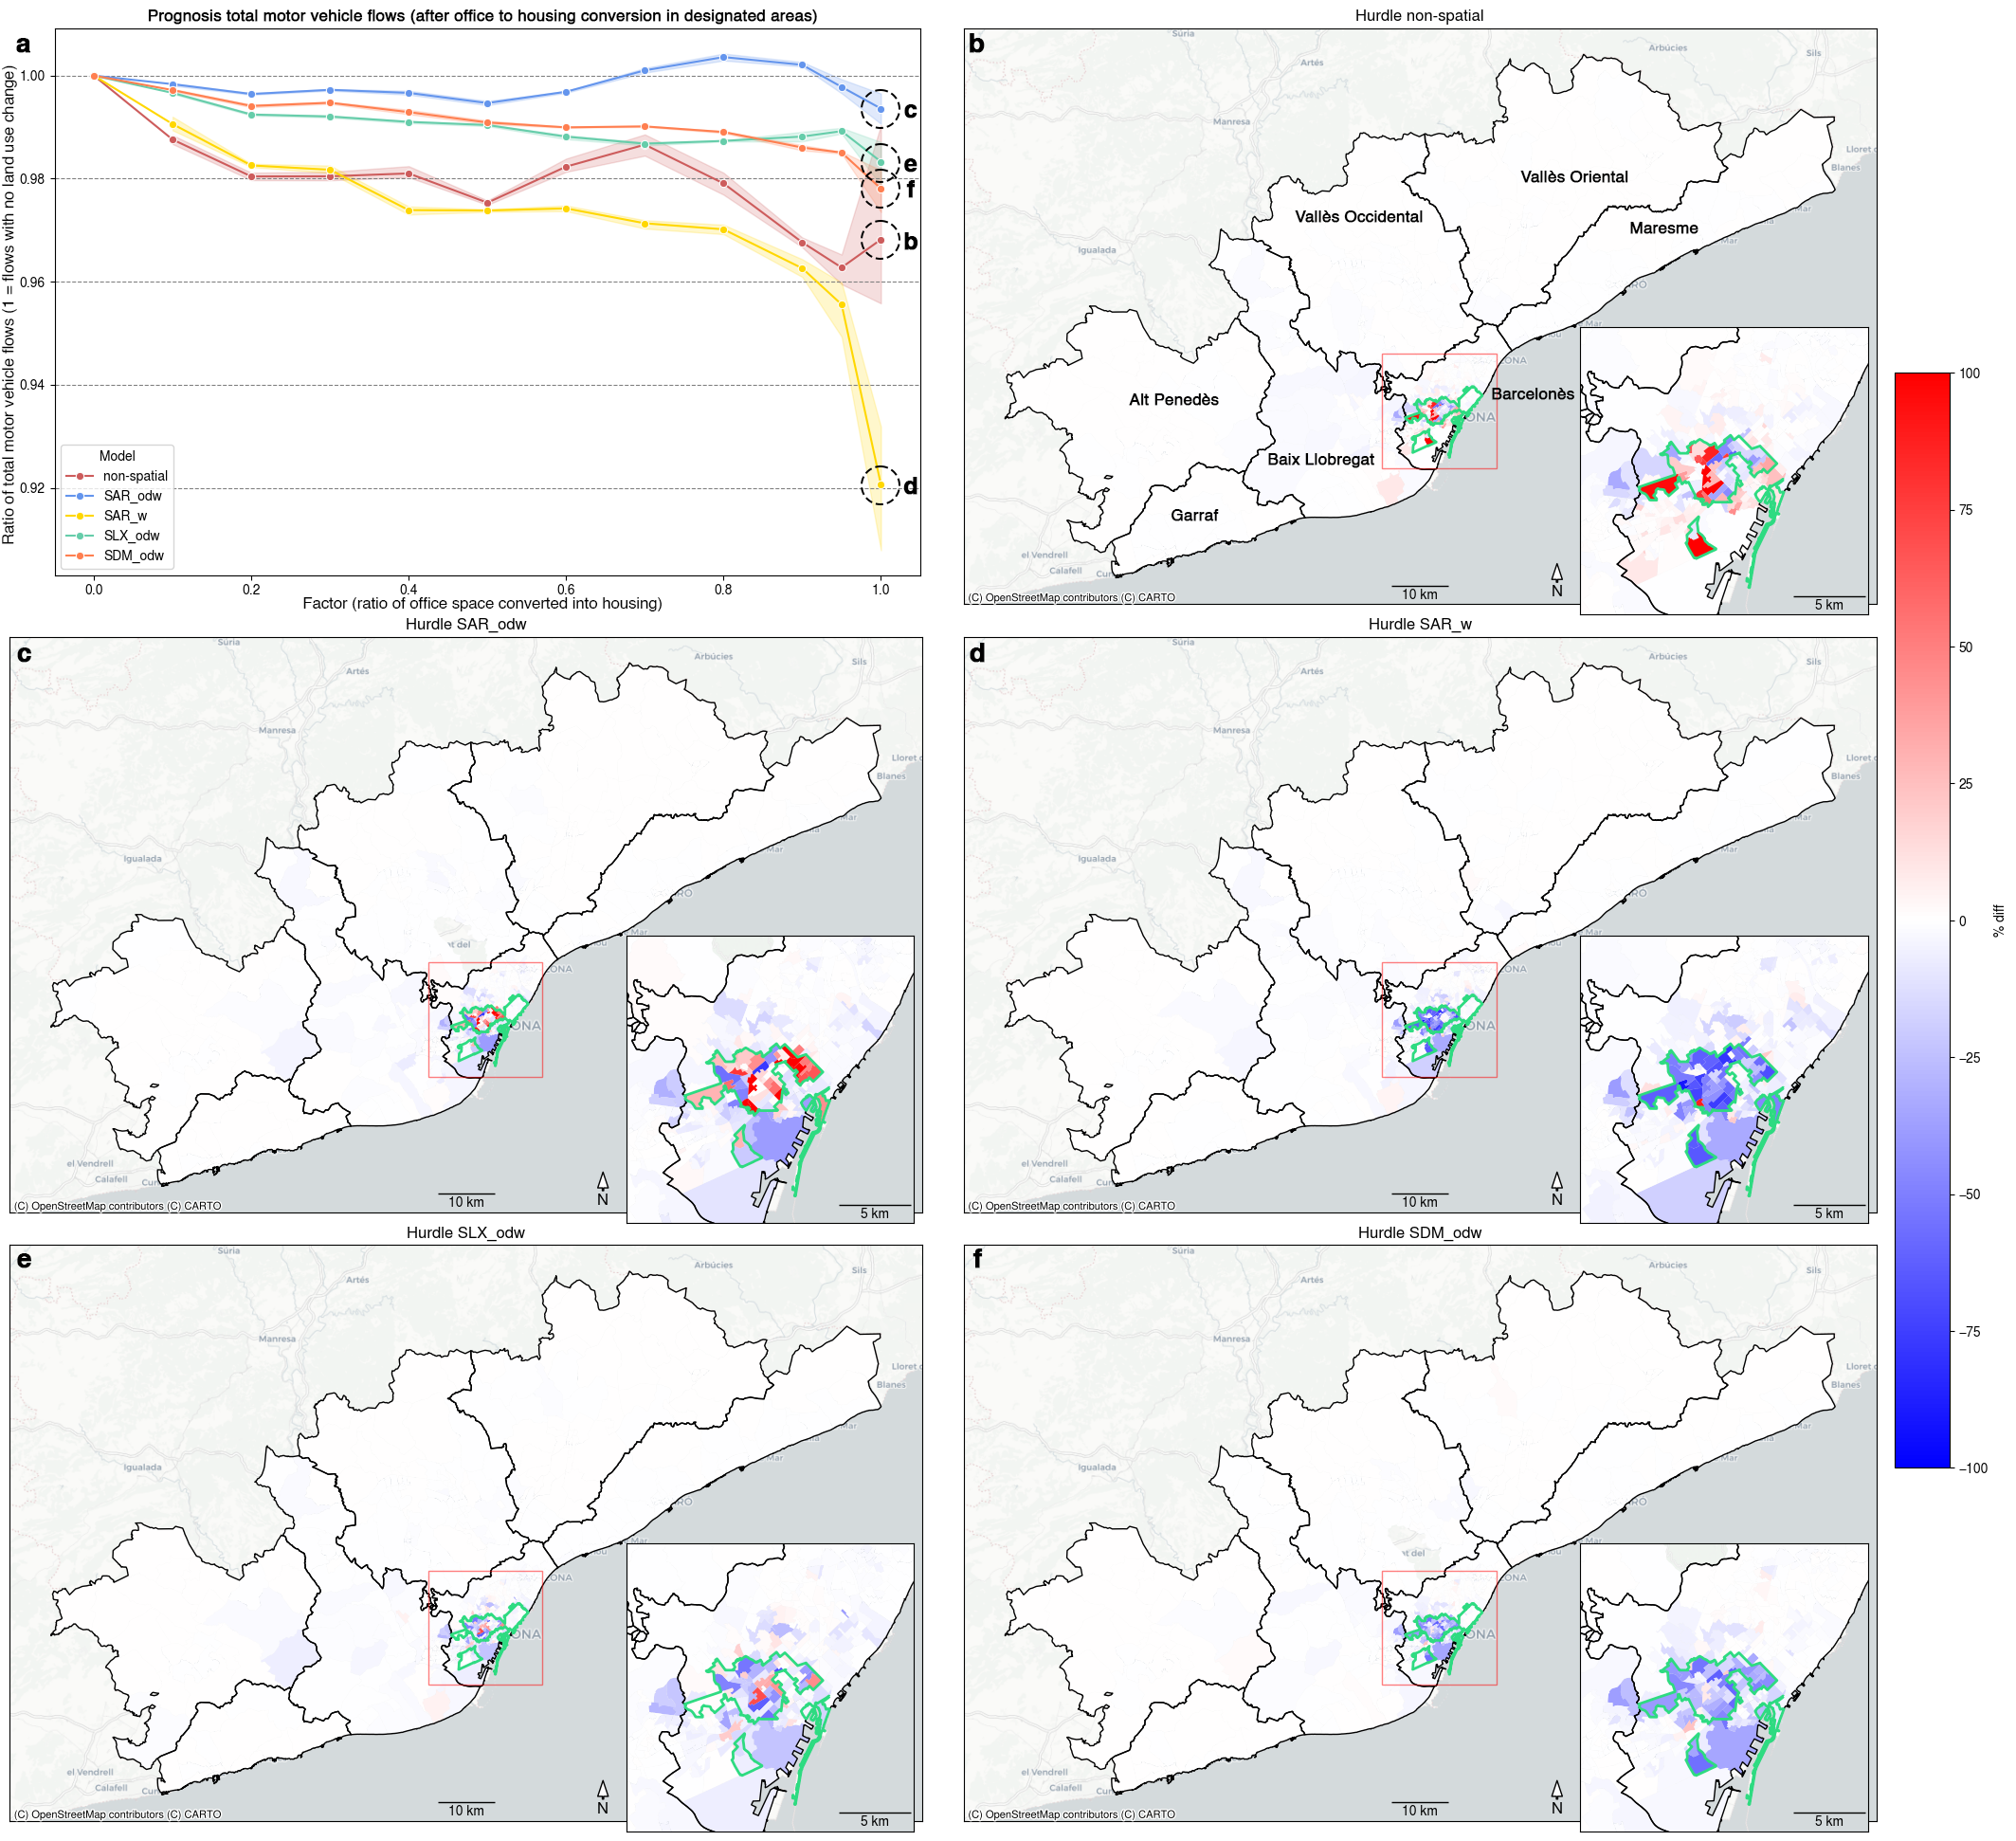
\includegraphics[width=1\textwidth]{fig_prognosis_combined_v1 copy.png}
    \caption{Prognosis study of conversion from office to residential use in selected areas of the RMB. Subpanel \textbf{a} shows the ablation study across different specifications (\textbf{b}-\textbf{f}) of the two-part Hurdle model, i.e. the impact on the total vehicle trips generated for the RMB by converting offices into residential space at different \emph{factor} ratios, where $\mathit{factor}=0.0$ corresponds to no conversion at all and $\mathit{factor}=1.0$ means the transformation of all offices into residential space. The bands represent the 95\% confident intervals resulting from introducing a $\pm2\%$ disturbance. Subpanels \textbf{b}-\textbf{f} show the generated vehicle trips by the different models with $\mathit{factor}=1.0$ at the level of each zone. The inset zooms into the city of Barcelona. The zones where the transformation from office to residential use has been applied are highlighted in green. Solid black lines indicate county borders (\textit{comarques}).}
    \label{fig:prognosis_summary}
\end{figure*}

The 44 zones of the RMB, where the office-to-housing transformation is applied, are central to the RMB (marked in green in Figure~\ref{fig:prognosis_summary}b-f). They do not include the most representative and premium locations for offices in the city \citep{EYStrategyandTransactions2023The2023}. However, despite the relatively small extension, they account for almost 20\% of the office space in the RMB, with a larger-than-average mean office unit size (Table~\ref{tab:intervention_area_characteristics}).

The different model specifications predict slightly different outcomes (see Figure~\ref{fig:prognosis_summary}a). Almost all of them agree on a dropping transportation demand trend with the increase of the offices converted into housing (i.e. $\mathit{factor}$), except for the $\text{SAR}_{i=o,d,w,}$, which tends to be unaffected by the conversion of offices, and fluctuates around the reference value. Notably, $\text{SAR}_{i=w}$ shows a drop of up to 8\% of total vehicle trips for a complete conversion ($\mathit{factor}=1.0$).  More conservative forecasts are provided by the non-spatial models, $\text{SLX}_{i=o,d,w}$ and $\text{SDM}_{i=o,d,w}$, with a drop of vehicle traffic in the range of 2-3\%. 
Particularly interesting is the behavior of the forecast when $\mathit{factor}>0.9$, 95 \% CI broadens in all the models, suggesting some unexpected effects caused by the total replacement of offices. 
Particularly, whereas the non-spatial model tends to forecast more vehicle trips when $\mathit{factor}\rightarrow1.0$, $\text{SAR}_{i=w}$ predicts a strong drop. Despite the differences, there is an agreement on the reduction of overall traffic demand, when office space is converted into residential use despite the related increase in the population.
Additionally, SAR specifications show varying outcomes, with reductions ranging from 1\% for \(\text{SAR}_{i=o,d,w}\) to 8\% for \(\text{SAR}_{i=w}\).

\section{Discussion}
\label{sec:ETRCO2H_Discussion}

As expected, no single factor can account for the entire heterogeneity and diversity of human mobility. Various elements, including topology and urban structure, population density, and activity features, among others, play crucial roles. Socio-demographic and cultural factors also significantly impact urban mobility \citep{Noulas2012AMobility}. Understanding these factors helps operationalize research and leverage the resulting insights to inform planning. This enables the orientation of urban dynamics in a favorable direction while mitigating undesirable effects such as congestion, resource misallocation, and adverse societal, psychological, economic, or personal consequences.

Teleworking and remote work can spread working locations across larger areas rather than concentrating them, and also encourage the creation of more hybrid and mixed-use spaces. This increased complexity makes it necessary to develop new tools allowing one to understand, model, and plan how cities operate \citep{Camocini2011TeleworkingWorkplace}. Zoning and strict separation of functions, which have often determined contemporary cities in search of urban optimization, have been intensively criticized for exacerbating transportation needs as well as for denaturalizing the mixed and complex interactions of urban systems \citep{Jacobs1961}. Whereas the development of contemporary transportation has allowed cities to grow beyond the human locomotion limits, it is still an open question how to find effective tools and methods in urban planning to leverage the distribution of uses across the territory with transportation (including energy and time) requirements.

These complex interactions of different urban factors make it challenging to anticipate the outcomes of policies and planning decisions with a simple qualitative assessment. The renovation, update, and redefinition of existing built-up areas in cities become critical because of socio-economic shifts (e.g. deindustrialization, production and energy transitions, socio-demographic changes, accumulation of capital in some locations, etc.) and environmental reasons aiming to ensure sustainable urban growth while avoiding expansive new developments and over-sprawling \citep{Kahn2000TheSuburbanization,Holden2004EcologicalForm,Echenique2012GrowingSustainably} as part of undergoing changes in cities.
This internal renovation of cities and update in land use also relate closely to densification challenges \citep{Wicki2022AcceptingNeighbourhoods}. These involve acceptance and political feasibility, which are deeply entangled with the underlying motivations, local contexts, tangible effects on urban life quality, and the capitalization of social and economic costs and benefits \citep{Zografos2020TheProject}. Therefore, they require a holistic consideration  \citep{Wicki2024OffentlicheInnenverdichtung} that should be nevertheless common to any urban intervention. 

Densification is often perceived as a risk to the quality of life due to oversaturation, gentrification, and displacement \citep{Rerat2010NewDebates, Chapple2017IncomeDisplacement} hindering social sustainability. However, it can also increase housing stock in some degree and facilitate access to services \citep{Neuman2005TheFallacy, Bramley2009UrbanType}. Simultaneously, commercial and office space may be losing occupation and value due to teleworking and e-commerce \citep{Le2022ImpactsReview}, which move part of human activity to virtual, digital environments. Not to mention that new working habits and organizational structures may outdate existing building supply, both qualitatively (i.e. design-wise) and quantitatively (due to a lack of match of spatial supply and demand). Stricter and more demanding building codes may require updating and renovating existing structures, which can be seen as an opportunity to reconsider their use. 
However, the results of our models indicate that the office built-up area has a subtle effect on the general vehicle mobility patterns. Based on our results, we expect that the conversion into residential space would affect the vehicular traffic flow patterns, but not that much. Counterintuitively, it is even predicted to reduce traffic flow between zones.
Accordingly, population increase does not necessarily imply more vehicle traffic as the reduction in office supply may be linked to hybrid work settings, increased home-office, shorter trips, and less job-related commuting.

Economic factors are the main drivers for the adaptive reuse of offices into housing, which determine the buildings and areas that should be renovated or should be subject to change of use to accommodate and exploit emerging needs and trends.
However, these transformative processes face legal, financial, technical, functional, and cultural challenges \citep{Remy2014}.
Also, gaining public acceptance for such changes is another challenge. Therefore, it is usually then up to public authorities and local communities to decide how to manage these demands. It is in this context that our research hopes to facilitate improvements. It aims to support the decision-making process by revealing likely outcomes. Thereby, it can contribute to clarifying and reducing the uncertainty of the effects of urban planning, which may obstruct the acceptance and feasibility \citep{Wustenhagen2007SocialConcept}. Providing new insights into the results of complex interactions in urban systems that otherwise would be hard to apprehend, can help to operationalize the exploration of alternatives for future cities transparently and understandably for all involved stakeholders. This is a valuable feature that could be easily integrated into larger frameworks of participatory city-making and accountable use of urban digital twins \citep{Helbing2023, Bettencourt2024RecentTwins, Ferre-Bigorra2022TheTwins}. 

The use of computer models has a long tradition in urban planning \citep{Wegener2021Land-UseModels}. Autoregressive (SAR) models have been widely used in literature to estimate and predict OD flows. However, the definition of spatial lags ($W$) may be challenging, and hence, this approach requires a few considerations:
\begin{enumerate}
    \item It builds on a stationarity assumption, meaning that the spatial relationships stay relatively constant over time, which may not be always accurate. 
    \item The spatial weights should be updated for the new predicted flows, resulting in different spatially lagged values. 
\end{enumerate}
Thus, an adaptive weighting approach and dynamic modeling are needed to account for the feedback process between new predictions and derived lagged variables. Additionally, the different specifications for the spatial filtering of the lags of the dependent variable can result in very different outcomes (e.g. compare the different forecasts in Figure~\ref{fig:prognosis_summary}a for $\text{SAR}_{i=o,d,w}$ and $\text{SAR}_{i=w}$). While specifications for autoregressive (SAR) models may yield slightly smaller errors, their extrapolation and forecasting capabilities can be compromised, as shown with the wider ranges of possible outcomes in Figure \ref{fig:prognosis_summary}a, especially in cases of over-specification with $i=o,d,w$ \citep{Griffith2020SomeModels}.

Alternatively, the SLX model, i.e. with spatial lags of $X$,  can provide a feasible and easier-to-implement approach, resulting in a similar prediction accuracy without requiring additional assumptions about data updating for the spatial lags (see Table~\ref{tab:all_model_stats}). Additionally, all of the considered specifications for the two-part Hurdle model show a similar spatial structure of the errors (see Figure~\ref{fig:maps_4models_perfectage_error_generated}). The main difference seems to be in the magnitude of these errors. Further advantages of the SLX model over other spatial econometric models are the full flexibility to account for spatial spillovers and the possibility of using conventional techniques to test for potential endogeneity \citep{Elhorst2022TheBar}. In general, all modeling approaches and spatial interaction specifications agree, indicating that the characteristics of neighboring zones are significant in predicting vehicle flows. 
% Particularly, in the case of vehicle flows, spillover effects seem intuitive. 
Particularly, in the center of compact cities, vehicle trips usually do not precisely account for the complete point-to-point trips, and the starting and end points of the motorized leg of the trip will likely not match with the origin and destinations that motivated the trip. These could be in different zones, making spillover effects even more relevant when modeling vehicle mobility.

\begin{figure*}[h!]
    \centering
    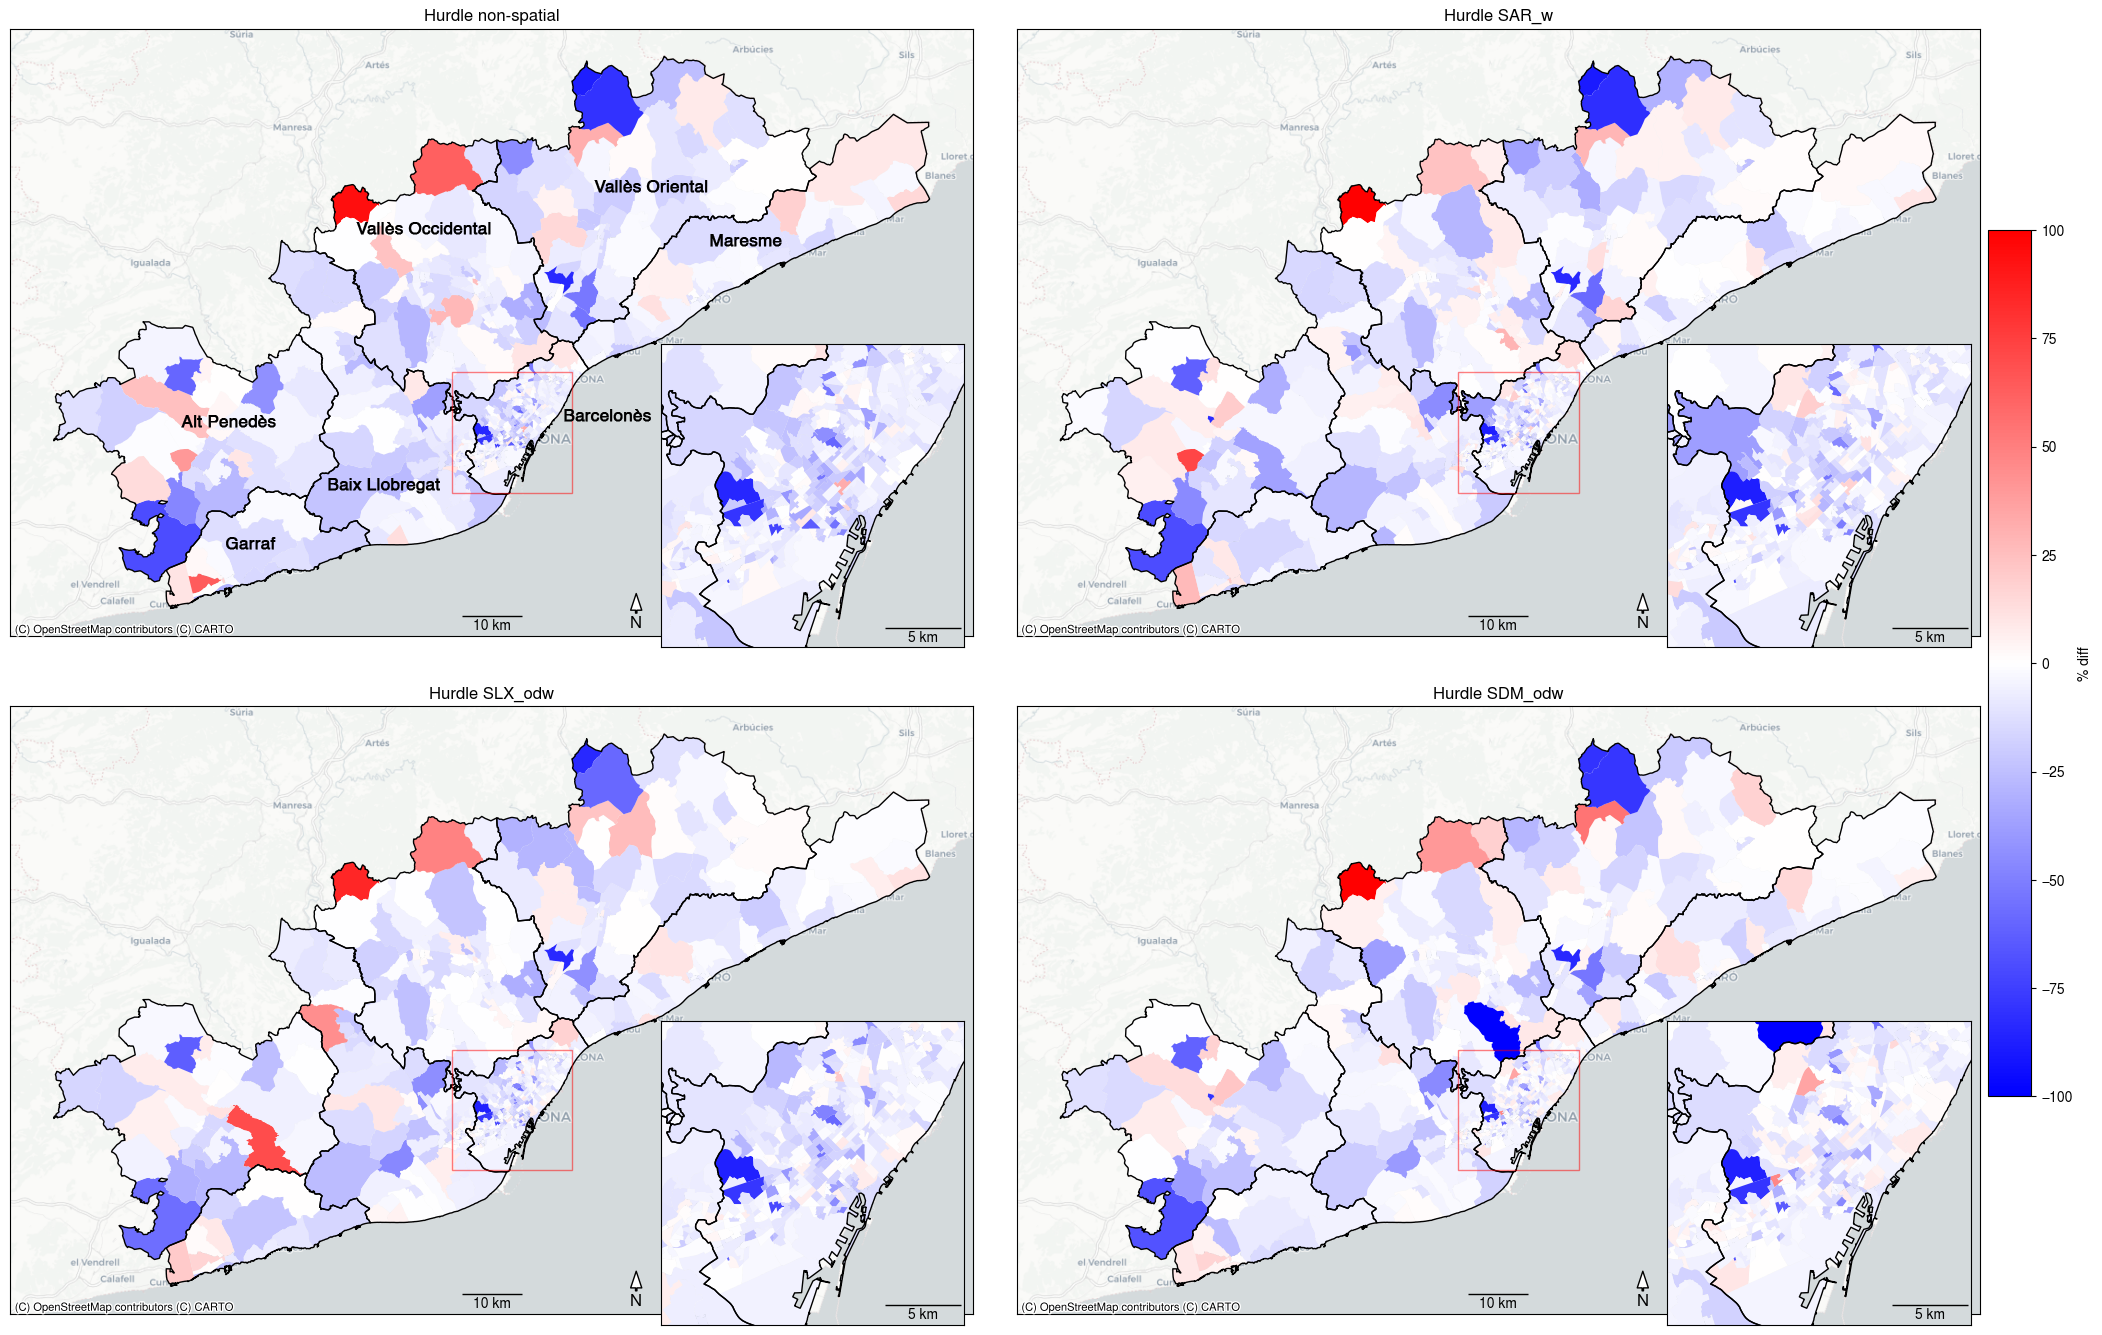
\includegraphics[width=1\textwidth]{fig_generated_perc_diff_SDM_v4.png}
    \caption{Comparison of the four most competitive models based on their percentage error for the total generated vehicle trips for each zone in the RMB. The inset zooms into the city of Barcelona. Solid black lines indicate county borders (\textit{comarques})}
    \label{fig:maps_4models_perfectage_error_generated}
\end{figure*}

Also, the results from the application of the model in Figure~\ref{fig:prognosis_summary} show that the forecasted reduction of motor vehicle traffic may stop or even increase when almost all the offices are converted into housing (i.e. $\textit{factors}>0.95$). Although further research is needed, these results suggest some unexpected effects, potentially related to the lack of mixed land use areas.
Nonetheless, the proposed model can estimate and forecast robustly the whole measured demand with the potential complexity involved. 

\section{Limitations and outlook}
\label{sec:ETRCO2H_Limitations}

The presented research focuses on land use, socio-demographics, and vehicle mobility in the case of inner-city renovation and building adaptive reuse \citep{Remy2014}. This scope could be further expanded to introduce multi-modality and environmental impacts \citep{Wegener2021Land-UseModels, Acheampong2015LandDirections, Rodriguez-Rey2022ToQuality}, also through complementary microsimulation \citep{ArgotaSanchez-Vaquerizo2023LessCity-making}. Additionally, factors regarding transport policies could be considered, particularly concerning changes in costs of transportation \citep{Guzman2014OptimalScheme}, to assess their impact on urban structure, on citizen behavior, and ultimately on their quality of life. Note, furthermore, that the modeling approach %, as it has been previously remarked for utility-based models, 
is not focused on the behavioral and decision-making processes at the individual level involving uncertainty \citep{Rasouli2014ApplicationsResearch}. Particularly, further research is needed regarding preferences toward hybrid work arrangements \citep{Heimgartner2024HybridFrequencies}. 
The formulation of such approaches would require much higher complexity \citep{Acheampong2015LandDirections} and novel approaches toward practical policy-making or participatory decision-making processes with non-experts \citep{Carteni2022ALevels}.

While spillover effects have been found to be statistically relevant and useful to improve predictions through lagged variables, from an empirical point of view the specification of the weight matrix $W$ defining the spatial interactions is weak \citep{Costantino2023AItaly}. As spatial weight specifications have an important impact on the models' performance, future work may explore additional alternatives not considered in this paper such as a different variable selection, non-symmetric lags included simultaneously at origin and destinations, or expanding variables through spatial feature engineering and using other databases connected to real estate or historical dataset on teleworking trends. This will contribute as well to studying the generalization of the approach to different locations. 

The proposed interventions considered in the prognosis results used very conservative assumptions about which could be the related socio-demographic changes due to the land use shift from commercial buildings to housing based on preserving the main characteristics of the affected zone: e.g. same average age, the same average size of residential units, etc. Beyond the simple change of land use, policy making, urban planning, building codes, and other planning resources allow the design of more detailed strategies that could have different effects. Incentivizing changes in the socio-demographics of dwellers of a given area or household size, among other factors, could have different impacts than those envisioned by these results. It means, that transforming offices into residential spaces may have a different impact by controlling for aspects of the implementation. The existing models didn't find any relevant and significant effect in factors such as age, income, or gender proportion in the zones to explain vehicle flows. However, they may affect preferences for teleworking, as well as the cost of housing may impact the type of demographics that may densify an area. Also, it is important to consider more distant effects. Our results show that located transformations in the core of the city will have as well an impact in distant zones of the metropolitan area, even not directly connected to the city (Figure~\ref{fig:3d}).

\begin{figure*}[h!]
    \centering
    \includegraphics[width=1\textwidth]{3d_fig_b copy.jpg}
    \caption{Changes in population density and vehicle flows between zones for different models after converting all offices into housing ($\mathit{factor}=1.0$). Models: (\textbf{b}) non-spatial interactions, (\textbf{c}) $\text{SAR}{i=o,d,w}$, (\textbf{d}) $\text{SAR}{i=w}$, (\textbf{e}) $\text{SLX}{i=o,d,w}$, and (\textbf{f}) $\text{SDM}{i=o,d,w}$. Zones where the transformation is applied are highlighted by an increase in population density, represented by extruded bars in red tones (\textbf{a}). Changes in OD motor vehicle flows are represented as arcs, with transparency indicating the relative change from the initial value—red hues for increases and blue for reductions in traffic. Only the top 500 OD pairs with the largest changes in vehicle flow between zones are shown. The inset zooms into the city of Barcelona. Solid black lines indicate county borders (\textit{comarques}).}
    \label{fig:3d}
\end{figure*}

Additionally, we cannot ignore two problems linked to modelization. First, different spatial zoning may lead to somewhat different results.  \citep{LeSage2010SpatialFlows}. Second, the construction of the car OD flows as a dependent variable is based on the estimation method that transformed the original raw cell phone tracks into OD values of vehicle flows \citep{Calvet2020ObtencioM2019} which has not been used directly here. It is expected that the OD vehicle flows used may slightly differ from the OD matrix that would have resulted when applying a survey-based approach: 
\begin{enumerate}
    \item in the used OD matrix from cell phone tracks trips may be over-split if a trip had a stop longer than 1 hour, while a survey-based OD flow matrix may show that trip as a single one, and 
    \item in the used data, trips are more granularly recorded, such that every leg or stage of a given commuting flow, i.e. %home-work/other-home may 
   resulting in multiple trips recorded, whereas that same commuting flow would be recorded as a single one in a more conventional OD matrix. 
\end{enumerate}

Another added difficulty to model motor vehicle trips is based on its looser correlation to distance which makes it less sensitive to distance-based deterrence \citep{PerezSans2021}. 

Our approach tried to combine powerful statistical methods while keeping the approach accountable and explainable. 
%as possible as gradient boosting trees. 
The use of a two-part Hurdle model is the most successful identified approach to address the inflation of zero values in the data and reducing the error metrics. However, it may imply the presence of different mechanisms to define zero and non-zero values \citep{Cameron2013RegressionData}. 
Further research could implement deep learning techniques, as it has been done to improve the accuracy of gravity models \citep{Simini2021AGeneration}. Nonetheless, such approaches should be combined with explainable AI to ensure accountability and agency as part of potential policy-making processes. 

\section{Conclusion}
\label{sec:ETRCO2H_conclusion}


The main focus of this research is two-fold: 
\begin{enumerate}
    \item Proposing a spatial econometric model based on lags of exogenous variables \emph{X}, i.e. SLX model, using a two-part Hurdle model with a gradient boosting algorithm, for estimating and forecasting vehicle flows in OD matrices within the metropolitan region of Barcelona using a combination of socio-demographic, land use and topological data.
    \item Illustrating how this model can be connected and operationalized to address existing policy and planning challenges in the city regarding inner urban renovation and land use changes in the context of densification due to the conversion of offices into housing.
\end{enumerate}

We proposed a regression based on a spatial econometric model using lags of the independent variables \emph{X} to model the OD vehicle flows that are empirically estimated from real cell phone data in Barcelona at the level of transportation assignment zones. To deal with overdispersion and zero-inflated OD vehicle flows, we adopted a two-part Hurdle model using gradient boosting with XGBoost and set a Tweedie regression as the objective to match the empirical distribution of the data better. As independent variables, we chose a combination of relevant socio-demographic, land use, and spatial features. Spatial interaction econometric models also allow us to flexibly consider the interactions between nearby zones through spatial filtering. Overall, the accuracy and errors of the SLX model  (MAE=6.09, RMSE=99.66) are similar to previously considered modeling approaches, including autoregressive models which require more complex and sophisticated, even questionable, assumptions about the data. Our modeling strategy also avoids the black box effect of deep learning techniques, which can be problematic in the context of accountability and inquiry about mechanisms affecting urban dynamics.

The modeling approach is then used to illustrate how it can provide support to address emerging challenges in urban planning. Changes in working culture such as home office and remote working affect requirements regarding the use of existing buildings and mobility patterns, hence, traffic. Simultaneously, such changes are relevant to other challenges such as the shortage of affordable housing, inner-city renovation processes, and issues connected to gentrification and urban quality. 
Applying the proposed spatial econometric models to urban densification caused by the conversion of offices into housing (as it is envisioned by common, \emph{business-as-usual} real estate-driven urban development) is not necessarily expected to cause an increase in traffic in these zones. Traffic demand may even go down. Beyond this practical insight, the application of the discussed models highlights how these modeling approaches can be useful and valuable for decision-making in cities. 
\begin{enumerate}
    \item They are practical and valuable for providing insights from complex interactions that otherwise would be challenging to capture and that even can challenge intuitive assumptions. 
    \item Transparent modeling, which means, explainability and accountability of computer models is needed to provide an understandable rationale and some degree of certainty for stakeholders involved in the planning and decision-making process. 
    \item Altogether, these computational models can be integrated into planning processes with a reasonable effort, facilitating public participation and simulation within larger urban digital twin frameworks. 
\end{enumerate}

%TC:ignore
\FloatBarrier